\documentclass[10pt]{report}
%\documentclass[11pt,twoside]{report}%% for two-sided printing
\usepackage{helvet}
\renewcommand{\familydefault}{\sfdefault}
\usepackage{pdfpages,multicol,url}
\usepackage{amssymb,anysize,fancyhdr,graphicx,amsmath,multirow,bm,algorithm,algpseudocode}
\usepackage{placeins}
\usepackage{csthesis}
\usepackage{makeidx}  %%% standard INDEX
\usepackage[titletoc]{appendix}%%Ensure word appendix appears in toc
\usepackage[pagebackref=true,pdfstartview=FitH,bookmarksopen=false,colorlinks,linkcolor=black,citecolor=black]{hyperref}

\makeatletter
\g@addto@macro\bfseries{\boldmath}

\def\contentsline#1#2#3#4{%
  \ifx\\#4\\%
    \csname l@#1\endcsname{#2}{#3}%
  \else
    \csname l@#1\endcsname{%
      \hyper@linkstart{link}{#4}{#2}\hyper@linkend
    }{%
      % same link destination for the page:
      \hyper@linkstart{link}{#4}{#3}\hyper@linkend
      % link destination is the page itself:
      % \hyperpage{#3}%
    }%
  \fi
} \makeatother


\makeindex

%%% The following code demonstrates the ``other list'' facility. A new
%%% command \otherlist is defined for the List of Programs. Programs
%%% are defined as floating environments of type 3 (1 is used for figures,
%%% 2 for tables) and the information about them is stored in an
%%% auxiliary file with .lop extension. You can use this method to
%%% define several types of ``other lists,'' but in that case you'll
%%% need to add appropriate code to \lists in the csthesis.sty
%%% package.
%%% Note: It's better to move this code into your own mythesis.sty
%%% package. If you do that, you should get rid of the \makeatletter,
%%% \makeatother commands.
\makeatletter
\newcommand\otherlist{%
    \addcontentsline{toc}{chapter}{\otherlistname}
    \if@twocolumn
      \@restonecoltrue\onecolumn
    \else
      \@restonecolfalse
    \fi
    \chapter*{\otherlistname
      \@mkboth{\MakeUppercase\otherlistname}%
              {\MakeUppercase\otherlistname}}%
    \@starttoc{lop}%
    \if@restonecol\twocolumn\fi
    }
\newcommand*\l@program{\@dottedtocline{1}{1.5em}{2.3em}}
\newcommand\otherlistname{List of Programs}
\newcommand\programname{Program}
\newcounter{program}[chapter]
\renewcommand\theprogram{\thechapter.\@arabic\c@program}
\def\fps@program{tbp}
\def\ftype@program{3}
\def\ext@program{lop}
\def\fnum@program{\programname~\theprogram}
\newenvironment{program}
               {\@float{program}}
               {\end@float}
\newenvironment{program*}
               {\@dblfloat{program}}
               {\end@dblfloat}
\makeatother
%%% end of ``other list'' code

\begin{document}
\setlength{\pdfpagewidth}{8.5in}
\setlength{\pdfpageheight}{11in}
%%% set switches
%\contentspagefalse
\figurespagetrue
\tablespagetrue
\dedicationpagetrue
\quotationpagetrue
\otherlistpagetrue

%%% front matter
%% Copyright 1998 Pepe Kubon
%%
%% `titapp.tex' --- title and approval for thes-full.tex, thes-short-tex from
%%                  the `csthesis' bundle
%%
%% You are allowed to distribute this file together with all files
%% mentioned in READ.ME.
%%
%% You are not allowed to modify its contents.
%%

%%%%%%%%%%%%%%%%%%%%%%%%%%%%%%%%%%%%%%%%%%%%%
%
%   Title and approval pages
%
%%%%%%%%%%%%%%%%%%%%%%%%%%%%%%%%%%%%%%%%%%%%%

%%% title page

\title{Systematic Support of Parallel Bit Streams in LLVM}
\author{Meng Lin}
\qualification{B.Eng., University of Science and Technology of China, 2012}
\submitdate{Fall 2014}
\copyrightyear{2014}

%%% approval page


\chair{Dr.~Nick Sumner}

\signatory{Dr.~Robert D. Cameron,\\
       Professor,
       Computing Science,\\
       Simon Fraser University\\
       Senior Supervisor}

\signatory{Dr.~Thomas C. Shermer,\\
        Professor,
        Computing Science,\\
       %Simon Fraser University\\
       Supervisor}

\signatory{Dr.~Fred Popowich,\\
        Professor,
        Computing Science,\\
       %Simon Fraser University\\
       Supervisor}

\signatory{Dr.~Arthur (Ted) Kirkpatrick,\\
       Associate Director \& Professor,
       Computing Science, \\
       %Simon Fraser University\\
       External Examiner}

%%% generating title and approval pages
\beforepreface

 %% title, approval

%% Partial Copyright License (PCL)
%% Please check the library online regulations & Forms, http://www.lib.sfu.ca/thesis
\newpage
\addcontentsline{toc}{chapter}{Partial Copyright License}
\mbox{}
\makeatletter
\AddToShipoutPictureBG*{
            \setlength{\@tempdimc}{.06\paperheight}
            \setlength{\unitlength}{1pt}
           \put(\strip@pt\@tempdimb,\strip@pt\@tempdimc){
	
\includegraphics{PCL_Declaration.pdf}
	}
}
\makeatother
\newpage

%% Copyright 1998 Pepe Kubon
%%
%% `abstract.tex' --- abstract for thes-full.tex, thes-short-tex from
%%                    the `csthesis' bundle
%%
%% You are allowed to distribute this file together with all files
%% mentioned in READ.ME.
%%
%% You are not allowed to modify its contents.
%%

%%%%%%%%%%%%%%%%%%%%%%%%%%%%%%%%%%%%%%%%%%%%%%%%%
%
%       Abstract 
%
%%%%%%%%%%%%%%%%%%%%%%%%%%%%%%%%%%%%%%%%%%%%%%%%

\prefacesection{Abstract}
Here you put the abstract of the thesis.














 %% abstract
%%% Copyright 1998 Pepe Kubon
%%
%% `dedquot.tex' --- dedication and quotation for thes-full.tex from
%%                   the `csthesis' bundle
%%
%% You are allowed to distribute this file together with all files
%% mentioned in READ.ME.
%%
%% You are not allowed to modify its contents.
%%

%%%%%%%%%%%%%%%%%%%%%%%%%%%%%%%%%%%%%%%%%%%%%
%
%   Dedication/Quotation pages
%
%%%%%%%%%%%%%%%%%%%%%%%%%%%%%%%%%%%%%%%%%%%%%

\dedication{To whomever whoever reads this!}
\thesquot{%
``Don't worry, Gromit. Everything's under control!''\\[5pt]%
--- The Wrong Trousers, \textsc{Aardman Animations}, 1993%
}

%%% generate pages
\dedicquotation
 %% dedication and quotation, if any
%% Copyright 1998 Pepe Kubon
%%
%% `ack.tex' --- aknowledgments for thes-full.tex, thes-short-tex from
%%               the `csthesis' bundle
%%
%% You are allowed to distribute this file together with all files
%% mentioned in READ.ME.
%%
%% You are not allowed to modify its contents.
%%

%%%%%%%%%%%%%%%%%%%%%%%%%%%%%%%%%%%%%%%%%%%
%
%       Acknowledgment
%
%%%%%%%%%%%%%%%%%%%%%%%%%%%%%%%%%%%%%%%%%%

\prefacesection{Acknowledgments}

It is a great honor and pleasure for me to have my Master study in Simon Fraser University. I would like to give a big thank to Dr. Robert Cameron for all of his earnest instructions. I learnt a lot from him during these two years.

I would also like to thank Dr. Nick Sumner for his deep knowledge on LLVM and his great patience in assisting my thesis work. I would like to thank Dr. Thomas Shermer and Dr. Fred Popowich for early feedback on my thesis draft. I would like to give another big thank to Ken Herdy, who gave me a lot of support in those late nights in the lab. Nigel Medforth helped me with the experiments on icgrep as well as many instructions on the Parabix tool chain. Linda Lin helped me on Parabix tools too.

I would like to thank all the committee members for their precious time spent on my thesis. I would like to thank Simon Fraser University and Dr. Cameron again for providing me this awesome chance of studying computing science in Canada as well as providing financial support. I would like to thank my parents and all my friends in Canada that encouraged me and supported me during this journey.












 %%  acknowledgments

%%%  generate contents, lists of figures, etc.
\lists

%% preface (foreword), if any
%%% Copyright 1998 Pepe Kubon
%%
%% `preface.tex' --- preface for thes-full.tex from
%%                   the `csthesis' bundle
%%
%% You are allowed to distribute this file together with all files
%% mentioned in READ.ME.
%%
%% You are not allowed to modify its contents.
%%

%%%%%%%%%%%%%%%%%%%%%%%%%%%%%%%%%%%%%%%%%%%%%%%%%
%
%       Preface 
%
%%%%%%%%%%%%%%%%%%%%%%%%%%%%%%%%%%%%%%%%%%%%%%%%

\prefacesection{Preface}
Here go all the interesting reasons why you decided to write this thesis.



%%% prepare main section
\beforetext

%%% main matter
%%%%%%%%%%%%%%%%%%%%%%%%%%%%%%%%%%%%%%%%%%%%%%%%%
%
%       Chapter 1
%
%%%%%%%%%%%%%%%%%%%%%%%%%%%%%%%%%%%%%%%%%%%%%%%%

\chapter{Introduction}
\label{one}

Nowadays Single Instruction Multiple Data (SIMD) instructions are broadly built in for most commodity processors. Compared with the traditional Single Instruction Single Data (SISD) instructions, SIMD provides an intra-register form of parallel computing by performing the same operation on many elements at the same time \cite{Fisher_phd}. SIMD instructions are widely used for multimedia processing, digital signal processing or other compute-intensive applications \cite{multimedia_simd, dsp_simd}.

The recent method of parallel bit streams (Parabix) accelerates text processing using SIMD instructions, in applications such as UTF-8 to UTF-16 transcoding \cite{rob_u8u16, rob_u8u16_techreport}, XML parsing \cite{medforth_icxml, rob_xml} and regular expression matching \cite{rob_regex}. For these applications, byte streams of the input text characters are first transposed into 8 bit streams, one for each bit value of the character byte, and then loaded into SIMD registers so that 128 or 256 consecutive code units can be processed at once \cite{inductive_doubling_principle}. SIMD bitwise logic, shift operations, bit scans and other bit-based operations form the foundation of this programming model.

Although Parabix applications achieve substantial acceleration compared to sequential (SISD) equivalents, the Parabix tool chain needs to handle SIMD programming carefully. It is challenging for the following two major reasons:

\begin{enumerate}
  \item SIMD instruction varies greatly among different instruction-set architectures (ISAs) which makes it hard to write portable SIMD programs. Some operations in Intel SSE may not exist in PowerPC AltiVec and vice versa. For example, integer comparison intrinsic $pcmpgtq$ in SSE4 does not have correspondence in PowerPC AltiVec.
  \item Even within one specific SIMD instruction set, most operations are only available for some pre-chosen data sizes. This is referred as "sparse instruction set" in \cite{hybrid_simd_type_legalize} and they gave a good example: in Intel SSE4, to shift-left a vector was implemented, but to shift-right was not. The 32-bit and 16-bit shift operations were available, but 64-bit shift was not \cite{hybrid_simd_type_legalize}.
\end{enumerate}

The current Parabix tool chain uses the Inductive Doubling Instruction Set Architecture (IDISA) as an idealized computing model to overcome these two difficulties. Based on this model a library with the same name has been developed. It works well, but still has two shortcomings:

\begin{enumerate}
  \item IDISA requires different header files for different architectures. Although it has a uniform API for portability, each header depends heavily on target-specific implementation details to provide the best implementation of each operation.
  \item The IDISA generator \cite{hua_idisa} chooses the best implementation within the scope of a single function. This may be not the best when considering the context of this function. For example, when performing addition, we may know all the high bits of each field in a SIMD register is zero, making simplification possible.
\end{enumerate}

This motivates us to find a better back end and currently, the most promising back end framework is LLVM\@. LLVM promises to enable out-sourcing of low-level and target-specific aspects of code generation \cite{llvm_ghc, chris_msthesis}. Switching to LLVM back end benefits Parabix tool chain for the following:

\begin{enumerate}
  \item LLVM provides a target-independent intermediate representation (IR) with a vector-of-integer type system that matches IDISA requirement closely. Parabix operations can be expressed with IR and hence can be ported, in principle, to any platform that LLVM supports, including X86, ARM, PowerPC, MIPS, SPARC and many more.
  \item LLVM provides inter-procedural, whole program analysis and optimization \cite{llvm_cgo04}. By built-in type system in the low level representation, LLVM keeps more static information to the back end and help optimize Parabix operation with meaningful context.
  \item LLVM provides just-in-time compilation which allows runtime source generation. This is critical to some applications such as regular expression matching, which generates sequence of Parabix operations on the fly according to the input regular expression.
\end{enumerate}

However, the native back end of LLVM has a number of gaps in its support for parallel bit streams. SIMD support for 2-bit and 4-bit field width are not available; 1-bit field width is supported slowly. Packing high bits on 16-bit field width which is one of the four key elements in the IDISA model and critical for transposition does not lower to proper machine code on X86. In this thesis, we extend LLVM to systematically support parallel bit streams and achieve high-performance code generation on the X86 target. We make the following contributions:

\begin{itemize}
  \item We port the critical Parabix operations to the LLVM back end thus bringing all the benefit of LLVM discussed above into the Parabix technology.
  \item We redefine type legality in LLVM and extend LLVM type system with the inductive doubling principle so that vectors of small element type are properly supported.
  \item We insert logic in the LLVM back end to recognize and handle key Parabix operations. This allows efficient code generation while keeping the whole source code in target-independent IR\@.
  \item We add a dedicated LLVM intrinsic for the long stream addition and enable high-performance chained addition on the unbounded integer model which can be applied in broader applications.
  \item We evaluate the new LLVM back end with both micro benchmarks on single Parabix operation and application level profiles. We get the performance on X86 platform as good as the well-tuned IDISA library.
\end{itemize}

The remainder of this thesis is organized as follows. Chapter~\ref{two} provides a quick review of Parabix and LLVM\@. Chapter~\ref{three} shows the overall design goal; examples of the IR implementation are presented and compared with the IDISA library. Algorithms for machine code generation is discussed in Chapter~\ref{four} and the implementation details is in Chapter~\ref{five}. Chapter~\ref{six} evaluates our work with both per-instruction benchmarks and application level profiles. Chapter~\ref{seven} gives the conclusion.


%%%%%%%%%%%%%%%%%%%%%%%%%%%%%%%%%%%%%%%%%%%%%%%%%
%
%     Chapter 2
%
%%%%%%%%%%%%%%%%%%%%%%%%%%%%%%%%%%%%%%%%%%%%%%%%

\chapter{Background}
\label{two}

\section{SIMD and SWAR}
SIMD is a parallel computing concept that performs the same instruction on different data to exploit data parallelism. Most of today's commodity processors supports SIMD within a register (SWAR) and in the SWAR model, SIMD operations are applied within general-purpose or special registers and these registers are often partitioned into fields. Operations on each field are independent from any other fields, which means for example, carry bits generated by addition would not pass to the next field.

The other important feature of the SWAR model is that the partition is not physical but rather a logical view of the register, so that different views are available on the same register. For a 128-bit SIMD register, a valid partition can be sixteen 8-bit fields as well as four 32-bit fields. There is no penalty from switching the logical view and it is important since it enables the inductive doubling principle we would discuss later.

However, since the SWAR instruction sets for different platforms are developed independently and operations available are determined mostly by the application requirements, different platform has different SWAR implementation, and the available instructions set are often sparse in the sense that not every power-of-two field width are supported \cite{hybrid_simd_type_legalize}.

\subsection{Commercial SIMD Instructions Sets}
Some popular SIMD instructions sets are listed here:
\begin{itemize}
  \item Intel MultiMedia eXtension (MMX). It defines eight 64-bit registers known as MM0 to MM7 which are aliases of the existing IA-32 Floating-Point Unit (FPU) stack registers. MMX only provides integer operations for early graphical applications thus is not a general purpose instruction set for SIMD programming \cite{hua_idisa}.
  \item Intel Streaming SIMD Extensions (SSE) series. SSE extends the MMX instructions set and introduces eight new independent 128-bit SIMD registers known as XMM0 to XMM7. Its successor SSE2 adds a rich set of integer instructions to the 128-bit XMM registers which makes it a useful SIMD programming model. AMD added support for SSE2 in its AMD64 architecture soon after the Intel released SSE2 thus in effect making SSE2 broadly available across the desktop computers. We would use SSE2 as our main instructions set target for 128-bit registers. Intel then released SSE3, SSSE3, SSE4 and AMD released SSE4a as the following SSE generations.
  \item Intel Advanced Vector Extensions (AVX). AVX extends the size of SIMD registers from 128 bits to 256 bits and introduces 16 new registers YMM0 to YMM15. It fully supports SSE instructions and more importantly, shifts the two-operand operations towards the non-destructive three-operand form, which would preserve the content in operand registers and reduce the potential movement of data between registers. AVX supports a number of floating point operations on 256-bit registers and its successor AVX2 fills the gap of integer operations and ensures the transition from SSE to AVX instructions with the same programming model. AVX2 is available on the Intel Haswell architecture, and we use it as our main 256-bit target. AVX512 as the next generation AVX has been announced to support 512-bit SIMD registers.
  \item ARM NEON\@. ARM as a popular mobile platform introduces its own SIMD extension named NEON in their Cortex-A series processors. It has thirty-two 64-bit registers (D0 to D31) as well as sixteen 128-bit registers (Q0 to Q15). In fact, $D_{2 \times i}$ and $D_{2 \times i + 1}$ are mapped to the same physical location of the register $Q_i$ and some operations like multiplication on the 64-bit D registers can return result in the 128-bit Q register \cite{hua_idisa}. NEON supports the field width of 8 bits, 16 bits, 32 bits and 64 bits integer operations as well as 32-bit floating point operations.
\end{itemize}

\section{Parabix Technology}
Parabix technology is a programming framework for high-performance text processing that can utilize both SIMD and multi-core parallel processing facility. It is built on top of the parallel bit streams concept. Byte-oriented input stream is first transposed into 8 bit streams with each stream corresponds to one bit location in the byte stream. For encodings that requires more than one byte, more bit streams can be introduced and in each bit stream, we would have 1 bit of the code unit from the input. Figure~\ref{figure:streams} gives an example of the transposition, $B_0$ to $B_7$ are the bit streams of the ASCII encoded input data and zero bits are marked as periods (.) for clarity.

\begin{figure}[tbh]
\begin{center}
\begin{tabular}{cr}\\
input data  & \verb`a453z--b3z--az--a12949z--ca22z7--`\\
$B_7$ & \verb`.................................`\\
$B_6$ & \verb`1...1..1.1..11..1.....1..11..1...`\\
$B_5$ & \verb`111111111111111111111111111111111`\\
$B_4$ & \verb`.1111...11...1...111111....1111..`\\
$B_3$ & \verb`....111..111.111...1.1111....1.11`\\
$B_2$ & \verb`.11..11...11..11....1..11.....111`\\
$B_1$ & \verb`...11..111...1....1...1..1.1111..`\\
$B_0$ & \verb`1.11.11.1.111.1111.1.1.1111...111`\\
\verb:[a]: & \verb`1...........1...1.........1......`\\
\verb:[z9]: & \verb`....1....1...1.....1.11......1...`\\
\verb:[0-9]: & \verb`.111....1........11111.....11.1..`
\end{tabular}
\end{center}
\caption[Basis and Character Class Streams]{Basis and Character Class Streams. Cited from \cite{rob_regex}.}
\label{figure:streams}
\end{figure}

After the transposition, the character class bit streams would be generated using bitwise logic, e.g.\ \verb:[a]:, \verb:[z9]: and \verb:[0-9]: in the figure. With SIMD operations on the 128-bit register, 128 input code unit can be classified at the same time. Parabix defines a set of primitives on the arbitrary length bit stream, called the \textit{Pablo Language} which is usually applied on the character class bit streams to generate a number of \textit{Marker Streams}. Marker Streams mark meaningful locations such as where a tag starts and ends in the XML document and matching positions of a partial regular expression. A simple counting or scanning through the marker streams are usually the final step in the Parabix technology.

Some useful Pablo primitives are listed as the following \cite{rob_xml_2011}:
\begin{enumerate}
    \item Bitwise logic: AND, OR, XOR and NOT on arbitrary length bit stream.
    \item Advance: shift forward the whole bit stream for 1 bit. In a little ending system, shift forward is to shift left because the bytes that comes first in the input stream resides in the lower memory address.
    \item ScanThru: $s(M, C)$ denotes the operation of scanning from the marker stream $M$ as the initial positions through the spans of ones in the stream $C$. Figure~\ref{figure:scanthru} shows an example of it.
      \[ s(M, C) = (M + C) \land \lnot C \]
      One example of ScanThru is in XML well-formedness checking, to check if a {\tt <tag>} is written in correct syntax, $M$ would mark all the start positions of tags e.g.\ the next position after the opening angle bracket ({\tt <}) and $C$ is the marker stream for all legal tag content. $s(M, C)$ should mark all the positions of the closing angle bracket ({\tt >}) which close tags. Say $M_0$ denotes the character class of {\tt >}, then if $s(M, C) \land \lnot M_0$ is not all zero, some tag is not closed properly with the {\tt >} symbol. Note that all the tags in the stream are checked at once in parallel in the unbounded bit streams model.
    \item MatchStar: $m(M, C)$ returns all positions that can be reached by scanning from the initial positions marked in $M$ along the spans of ones in the stream $C$ for zero or more steps. MatchStar gets its name from the star operator (*) in the regular expression and it also has important application in the long stream addition. Figure~\ref{figure:matchstar} shows an example of it.
\end{enumerate}

\begin{figure}[tbh]
\begin{center}
\begin{tabular}{cr}\\
input data  & \verb`----173942---654----1----49731----321--`\\
$M_0$ &                          \verb`....1........1......1......1...........`\\
$D = $\verb:[0-9]: &             \verb`....111111...111....1....11111....111..`\\
$M_0 + D$ &                      \verb`..........1.....1....1...11...1...111..`\\
$M_1 = (M_0 + D) \wedge \neg D$ &\verb`..........1.....1....1........1........`
\end{tabular}
\end{center}
\caption[ScanThru Using Bitstream Addition and Mask]{ScanThru Using Bitstream Addition and Mask. Cited from \cite{rob_xml_2011} and slightly modified.}
\label{figure:scanthru}
\end{figure}

\begin{figure}[tbh]
\begin{center}
\begin{tabular}{cr}\\
input data  & \verb`a453z--b3z--az--a12949z--ca22z7--`\\
$M_1$ & \verb`.1...........1...1.........1.....`\\
$C = \text{\tt [0-9]}$ & \verb`.111....1........11111.....11.1..`\\
$T_0 = M_1 \wedge C$ & \verb`.1...............1.........1.....`\\
$T_1 = T_0 + C$ & \verb`....1...1.............1......11..`\\
$T_2 = T_1 \oplus C$ & \verb`.1111............111111....111...`\\
$M_2 = T_2 \vee M_1$ & \verb`.1111........1...111111....111...`
\end{tabular}
\end{center}
\caption[MatchStar Using Bitstream Addition and Mask]{MatchStar primitive, where $M_2 = \text{MatchStar}(M_1, C)$. Cited from \cite{rob_regex}.}
\label{figure:matchstar}
\end{figure}

Pablo Language are defined over unbounded bit streams which of course need to be translated into a block-at-a-time processing for real applications \cite{rob_regex}. The Pablo compiler is used here for the translation and it will take care of the carry bits across block boundaries with a carry queue. A block-at-a-time C++ code would be generated as a result.

\subsection{IDISA Library}
To actually execute the C++ code, a set of runtime library is necessary. Dr. Cameron proposed the Inductive Doubling Instructions Set Architecture in \cite{inductive_doubling_principle} and claimed significant instruction count reduction in core parallel bit stream algorithm. As he wrote, "inductive doubling refers to a general property of certain kinds of algorithm that systematically double the values of field widths or other data attributes with each iteration."\cite{inductive_doubling_principle}. There are four key elements of this architecture:
\begin{itemize}
    \item A core set of binary functions on SIMD registers, for all field width equals to $2^k$. To work with parallel bit streams, the operation ADD, SUB, SHL, SRL and ROTL (rotate left) comprise the set.
    \item A set of \textit{half-operand modifiers} that make possible the inductive processing of field width $2W$ in terms of combinations of field width $W$. These modifiers select either the lower half of the field or the higher half.
    \item Packing operations that compress two vectors of field width $W$ into one vector of field width $W/2$. E.g.\ collecting all the higher half bits of fields from two vectors into one.
    \item Merging operations that produce one vector of field width $W$ with two vectors of field width $W/2$.
\end{itemize}

A C++ library is then developed after this model and it is called the IDISA library. To be clear, in the following sessions the abstract architecture will be called the IDISA model to distinguish from the IDISA library. An interesting fact about the IDISA library is that it is actually generated automatically from a pool of strategies to avoid duplicated human work among different targets. When targeting at a new platform, a set of machine intrinsic will be mapped to proper instructions in the IDISA model. This would be sparse that many other operations needed by the model are still not available. The IDISA library generator could fill the gaps with a pool of strategies which basically tells how to implement instruction C given instruction A and B are available. Multiple strategies for the same instruction may exist and the generator would choose based on least instruction count mechanism \cite{hua_idisa}.

\begin{figure}[ht!]
\centering
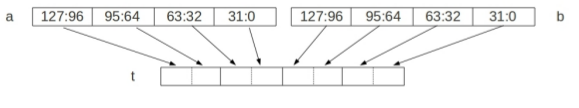
\includegraphics[width=130mm]{draw/horizontal.png}
\caption[Horizontal Operations in IDISA]{The logic of IDISA Horizontal Operations, cited from \cite{hua_idisa}.}
\label{figure:horizontal}
\end{figure}

\begin{figure}[ht!]
\centering
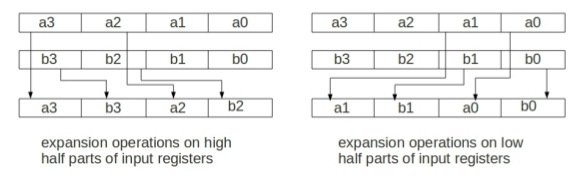
\includegraphics[width=130mm]{draw/expansion.png}
\caption[Expansion Operations in IDISA]{The logic of IDISA Expansion Operations, cited from \cite{hua_idisa}.}
\label{figure:expansion}
\end{figure}

The IDISA library divides SIMD operations in the following categories \cite{idisa_webpage}:
\begin{itemize}
    \item Vertical Operations (Template Class {\tt simd<w>}): Most common SIMD operations between two registers and {\tt w} is the field width. E.g.\ {\tt simd<8>::add(A, B)} aligns registers A and B vertically and adds up the aligned 8-bit fields. Different fields are independent of each other.
    \item Horizontal Operations (Template Class {\tt hsimd<w>}): Operations like packing align the two operands horizontally, extract a portion of the bits in operands and concatenate into one full SIMD register. (Figure~\ref{figure:horizontal})
    \item Expansion Operations (Template Class {\tt esimd<w>}): Operations that double the width of fields like merging which would take the higher 64 bits of the two operands (A and B), concatenate the first field from A and the first field from B and get a new field with the width doubled. Do the same to the following fields until a full SIMD register C is generated. (Figure~\ref{figure:expansion})
    \item Field Movement Operations (Template Class {\tt mvmd<w>}): Operations that copy and move the entire fields. The content of these fields would not change.
\end{itemize}

The IDISA library claims to have better performance compared to the hand-written libraries and it is the main competitor of our LLVM back end.

\subsection{Critical Parabix Operations}
There are at least three critical Parabix operations that can be the performance bottleneck and need special attention:
\begin{itemize}
    \item Transposition. The first step of every Parabix application and can be the primary overhead of some Parabix application. There are two major algorithms: the ideal three-stage implementation and the byte-pack implementation. The byte-pack implementation utilize packing on 16 bit field width which is widely available on commodity processors while the ideal three-stage implementation was proved optimal in instruction count in the IDISA model. Details of these two algorithms can be found in \cite{inductive_doubling_principle}.
    \item Inverse transposition. For some applications like the UTF-8 to UTF-16 transcoding, parallel bit streams needs to be modified and translated back into byte streams, thus an inverse transposition is needed. As the inverse operation to the transposition, there are also two algorithms available which mirror the transposition algorithms. A detailed discussion can be found in \cite{rob_u8u16}.
    \item Long stream addition. Pablo compiler deal with addition between unbounded bit streams using chained long stream additions, which adds two numbers as wide as the SIMD register with a carry-in bit and generates a carry-out bit. The naive approach would be chaining 64-bit additions together to emulate 128-bit, 256-bit or 512-bit additions. The time complexity of the naive approach grows linearly with the SIMD register size and a better algorithm is proposed in \cite{rob_regex} which could adds up to 4096 bits wide integers in constant time. We would discuss this algorithm further in Chapter~\ref{four}.
\end{itemize}

Since they are performance critical, these operations would be used as the application level benchmarks in the evaluation section.

\section{LLVM Basics}
The \textit{Low Level Virtual Machine (LLVM)} is an open-source, well developed compiler tool that is dedicated to the compiler writers. It is proposed in 2000 with Lattner's Master thesis \cite{chris_msthesis} and is gaining popularity ever after. Today it is developed into a high-performance static compiler back end with just-in-time compilers and life-long program analysis and optimization, which means program analysis and optimization in compile time, link time and run time \cite{llvm_ghc, llvm_cgo04}. It supports a variety of targets from Intel X86, PowerPC to the ARM mobile platform and hides the low-level target-specific issues for the compiler writers. LLVM is now sponsored by companies like Google and Apple and it is likely to become the default back end choice that last a long time in this field.

LLVM uses the intermediate representation (IR) as its virtual instruction set and IR is used as not only the input code to the LLVM tool chain but also the internal representation for analysis and optimization passes. This enables the programmer to use LLVM as a pipeline and inspect output from each step. Although IR is low-level, it preserves high-level static information through the strong type system and its static single assignment (SSA) form. According to \cite{cytron1991efficiently}, SSA form guarantees only one assignment to every variable and would help calculate the high-level data flow. The main design goal of IR is to be low-level enough so that most programming language can target to it while maintaining the most high-level information to make aggressive back end optimization possible \cite{llvm_ghc}.

LLVM IR is target-independent and it provides powerful operations like shufflevector that can express most of the complex Parabix operations. The IR code are processed through the target-independent code generator and the machine code (MC) layer to become the native machine code. We will describe the code generation process in detail in the next section as it is the major piece of logic we extend for parallel bit streams.

\section{LLVM Target-Independent Code Generator}
The first stage for code generation is Instruction Selection, which translates LLVM code into the target-specific machine instructions. After that, there are machine level optimization like live-interval analysis and register allocation. We focus on Instruction Selection and it is done by the following steps \cite{llvm_code_gen} (we would describe each step in the following text):

\begin{itemize}
  \item Initial SelectionDAG Construction: generate SelectionDAG from LLVM IR.
  \item DAG Combine 1
  \item Legalize Types Phase
  \item Post Legalize Type DAG Combine
  \item Legalize Phase
  \item DAG Combine 2
  \item Instruction Select Phase
  \item Scheduling and Formation Phase
\end{itemize}

LLVM internally constructs a graph view of the input code called SelectionDAG where DAG is short for directed acyclic graph. Each node in the DAG represents an operation with an opcode, a number of operands and a number of return values. If the DAG node A uses the return value of the other DAG node B, an edge will be there from B to A. The SelectionDAG enables a large variety of very-low-level optimization and also benefits the instruction scheduling process by recording the instruction dependency in the graph.

There are DAG combine passes after the initial construction and each legalize phase\cite{llvm_code_gen}. We will explain "legality" in the next section. DAG combine passes clean up SelectionDAG with both general and machine-dependent strategies, making the work easier for initial constructor and legalizers: they can focus on generating accurate SelectionDAG, good and legal operations with no worries of the messy output.

Instruction Select Phase is the bulk of target-specific logic that translates a legal SelectionDAG into a new DAG of target code with pattern matching facility. For example, a node of floating point addition followed by a floating point multiplication could be merged into one FMADDS node on the target that supports floating point multiply-and-add (FMA) operations \cite{llvm_code_gen}.

The Scheduling and Formation Phase would assign an order to each target instruction following the target's constraints. After that, a list of MachineInstrs will be generated and the SelectionDAG is no longer needed.

\subsection{Vector Type and Legality}
SIMD data are grouped into vectors and LLVM uses the notion \verb|<N x iX>| to represent a vector of N elements, where each of the element is an integer of X bits \cite{llvm_lang_ref, hybrid_simd_type_legalize}. \verb|<N x iX>| is also denoted as $vNiX$ as $vNiX$ is the internal type name used in the LLVM source code; e.g.\ \verb|<4 x i32>| is the same with $v4i32$.

In LLVM IR, programmer can write any kind of vectors, even $v1024i3$, and those vectors may not be supported by the target machine. LLVM has the notion of a "legal" vs. "illegal". A type is legal for a target only if it is supported by some operation. In SelectionDAG, a DAG node is legal only if the target supports the operation and operands type. For example, $v16i8$ is legal on X86 SSE2 architecture, since the architecture supports ADD on 2 $v16i8$ vectors; but it does not support multiplication on 2 $v16i8$ vectors, so that the DAG node MUL on $v16i8$ is illegal. LLVM has Legalize Types and Legalize Operations Phases to turn illegal type or DAG into legal\cite{llvm_code_gen}.

Legalize type phase has three ways to legalize vector types\cite{hybrid_simd_type_legalize}: \textit{Scalarization}, \textit{Vector Widening} and \textit{Vector Element Promotion}.

\begin{itemize}
    \item \textbf{Scalarization} splits the vector into multiple scalars. It is often used for $v1iX$ as the edge case when LLVM is trying to split the incoming vector into sub vectors.
    \item \textbf{Vector Widening} adds dummy elements to make the vector fit the right register size. It will not change the type of the elements, e.g.\ $v4i8$ to $v16i8$.
    \item \textbf{Vector Element Promotion} preserves the number of elements, but promote the element type to a wider size, e.g.\ $v4i8$ to $v4i32$.
\end{itemize}

After the type legalization, we may still have illegal DAG node, such as multiplication on $v16i8$ for X86 SSE2 architecture; thus we need legalize operations phase. There are three strategies in this phase:

\begin{itemize}
    \item \textbf{Expansion}: Use another sequence of operations to emulate the operation. Expansion strategy is often general in the sense that it may use slow operations such as memory load and store, but it would generate native code with correct outcome.
    \item \textbf{Promotion}: Promote the operand type to a larger type that the operation supports.
    \item \textbf{Custom}: Write a target-specific code to implement the legalization. Similar to Expansion, but with a specific target in mind.
\end{itemize}

No illegal type should be introduced in the operation legalization which puts a limitation on the machine-independent legalize strategies: $i8$ is the minimum integer type on X86 and programmer needs to extend every integer less than 8 bits to $i8$ before returning it to the DAG\@. On the other hand DAG combine is different, you can choose the combine timing on your own. If you choose to combine before Legalize Types Phase, you can freely introduce illegal types into your combined results.

\chapter{Design Objectives}
\label{three}

In this chapter we discuss about our overall goal for using LLVM as a new Parabix back end. First, we show that the IDISA library could be replace by a pure target-independent IR library.

To start, let us look at one IDISA vertical operation: {\tt simd<8>::add}. IDISA library implements this function with the compiler intrinsic that directly translates into the assembly code, so different header files have to be maintained for different instruction sets such as Program~\ref{prog:add_8_sse2} and Program~\ref{prog:add_8_neon}. However, with the LLVM IR, we can implement it as Program~\ref{prog:add_8_llvm}; no low level detail is specified here.

\begin{program}
\begin{verbatim}
  template <> bitblock128_t simd<8>::add(bitblock128_t arg1, bitblock128_t arg2)
  {
    return _mm_add_epi8(arg1, arg2);
  }
\end{verbatim}
\caption{Implementation of {\tt simd<8>::add} for X86 SSE2}
\label{prog:add_8_sse2}
\end{program}

\begin{program}
\begin{verbatim}
  template <> bitblock128_t simd<8>::add(bitblock128_t arg1, bitblock128_t arg2)
  {
    return (bitblock128_t)vaddq_u8((uint8x16_t)(arg1), (uint8x16_t)(arg2));
  }
\end{verbatim}
\caption{Implementation of {\tt simd<8>::add} for ARM NEON}
\label{prog:add_8_neon}
\end{program}

\begin{program}
\begin{verbatim}
  define <16 x i8> @simd_add_8(<16 x i8> %arg1, <16 x i8> %arg2) {
  entry:
    %r = add <16 x i8> %arg1, %arg2
    ret <16 x i8> %r
  }
\end{verbatim}
\caption{Implementation of {\tt simd<8>::add} with LLVM IR}
\label{prog:add_8_llvm}
\end{program}

\begin{program}
\begin{verbatim}
  define <16 x i8> @simd_eq_8(<16 x i8> %arg1, <16 x i8> %arg2) {
  entry:
    %r1 = icmp eq <16 x i8> %arg1, %arg2
    %r2 = sext <16 x i1> %r1 to <16 x i8>
    ret <16 x i8> %r2
  }
\end{verbatim}
\caption[Implementation of {\tt simd<8>::eq} with LLVM IR]{Implementation of {\tt simd<8>::eq} with LLVM IR. {\tt Sext} is the instruction for sign extension.}
\label{prog:icmp}
\end{program}

\begin{program}
\begin{verbatim}
  define <16 x i8> @simd_max_8(<16 x i8> %a, <16 x i8> %b) {
  entry:
    %m = icmp sgt <16 x i8> %a, %b
    %r = select <16 x i1> %m, <16 x i8> %a, <16 x i8> %b
    ret <16 x i8> %r
  }
\end{verbatim}
\caption[Implementation of {\tt simd<8>::max} with LLVM IR]{Implementation of {\tt simd<8>::max} with LLVM IR. {\tt Select} selects elements according to the first operand: $\text{\tt r}_i=
\begin{cases}
    \text{\tt a}_i& \text{if } \text{\tt m}_i = 1\\
    \text{\tt b}_i& \text{otherwise}
\end{cases}$.}
\label{prog:max}
\end{program}

Most of the IDISA vertical operations can be expressed with a few lines of IR code. A bit more examples are listed here:

\begin{itemize}
    \item Vector addition, subtraction, multiplication and shifting. There are IR instructions that correspond one-to-one with them.
    \item Integer comparison such as equality, greater than and unsigned less than. In IR, there is one instruction called `icmp' which does the comparison. The only difference is that for vector type {\tt <N x iX>}, the comparison result of `icmp' is in type {\tt <N x i1>} while IDISA requires it to be in type {\tt <N x iX>} (All ones in an element means true and all zeros means false). We need to perform a sign extension by coping the sign bit of the $i1$ result until it reaches the size of $iX$ (Program~\ref{prog:icmp}).
    \item Operations that have no IR correspondence such as {\tt simd::min} and {\tt simd::max}. They can be emulated with a sequence of IR, e.g.\ {\tt simd<8>::max} in Program~\ref{prog:max}.
\end{itemize}

For horizontal operations, IDISA also needs to maintain target-specific logic. For example, to implement {\tt hsimd<16>::packh}, it uses unsigned saturation $packuswb$ for X86 SSE2 and uses $vuzpq\_u8$ for NEON; for X86 SSE series after SSSE3, it uses the instruction $pshufb$. The author of the IDISA library needs to know these instruction sets very well. On the other hand, LLVM IR introduces a powerful instruction which can express most of the horizontal and expansion operations. It is the \textit{shufflevector}.

\begin{verbatim}
    <result> = shufflevector <n x <ty>> <v1>, <n x <ty>> <v2>, <m x i32> <mask>
    ; yields <m x <ty>>
\end{verbatim}

The first two operands are vectors of the same type and their elements are numbered from left to right across the boundary. In the other word, the element indexes are $0$ \ldots $n-1$ for {\tt v1} and $n$ \ldots $2n-1$ for {\tt v2}. The {\tt mask} is an array of constant integer indexes, which indicates the elements we want to extract to form the {\tt result}. Either {\tt v1} or {\tt v2} can be "undefined" to do shuffle within one vector. Shufflevector is often used together with the \textit{bitcast} operation. It converts between integer, vector and FP-values and changes the data type without moving or modifying the data, thus requiring the source and result type to have the same size in bits. With shufflevector and bitcast, we could write {\tt hsimd<32>::packh} in Program~\ref{program:packh_32}. Figure~\ref{figure:packh_32} explains the indexes used in the shuffle mask.

\begin{figure}[ht!]
\centering
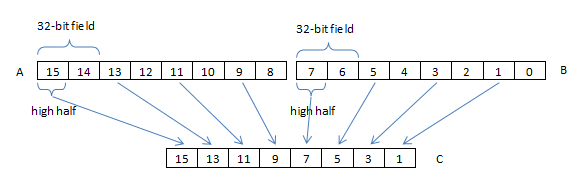
\includegraphics[width=130mm]{draw/packh_16.png}
\caption[Implement {\tt hsimd<32>::packh} with shufflevector]{Shufflevector and {\tt hsimd<32>::packh}. The vectors are bitcasted into $v8i16$ and the indexes for the shuffle mask are drawn in the cell.}
\label{figure:packh_32}
\end{figure}

\begin{program}
\begin{verbatim}
  define <8 x i16> @hsimd_packh_32(<4 x i32> %a, <4 x i32> %b) {
  entry:
    %aa = bitcast <4 x i32> %a to <8 x i16>
    %bb = bitcast <4 x i32> %b to <8 x i16>
    %rr = shufflevector <8 x i16> %bb, <8 x i16> %aa, <8 x i32> <i32 1, i32 3,
          i32 5, i32 7, i32 9, i32 11, i32 13, i32 15>

    ret <8 x i16> %rr
  }
\end{verbatim}
\caption[Shufflevector implementation of packh.]{Shufflevector and {\tt hsimd<32>::packh} in LLVM IR\@. Horizontal operations half the width of fields and that effect is reflected in the return value type.}
\label{program:packh_32}
\end{program}

Program~\ref{program:packh_32} can be easily generalized for packing high on any power-of-two field width. For other horizontal operations:
\begin{itemize}
    \item Packing low: the same bitcast need to be done but shufflevector with a different mask. For example, {\tt hsimd<32>::packl} can be implemented with the mask {\tt 0, 2, 4, 6, 8, 10, 12, 14}.
    \item Packing sign mask: it packs together all the sign bits from each field of the operand. This can be implemented with the less than comparison. For example, {\tt hsimd<32>::signmask(a)} is equivalent to \verb|icmp slt <4 x i32> %a, <4 x i32> <i32 0, i32 0, i32 0, i32 0>| which returns a {\tt <4 x i1>} sign mask vector.
    \item Other operations that require coding a sequence of IR like {\tt hsimd<32>::add\_hl(a, b)}. They are rarely used in the Parabix application.
\end{itemize}

Shufflevector and bitcast could also cover IDISA expansion operations. We list the IR code for {\tt esimd<16>::mergeh} in Program~\ref{prog:mergeh_16} and explain the indexes in Figure~\ref{fig:mergeh_16}. The program is self-explanatory; any programmer who understands shufflevector can understand its behaviour easily.

\begin{figure}[ht!]
\centering
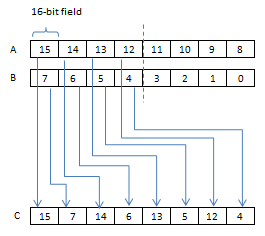
\includegraphics[width=60mm]{draw/mergeh_16.png}
\caption[Implement {\tt esimd<16>::mergeh} with shufflevector]{Shufflevector and {\tt esimd<16>::mergeh}. The indexes for the shuffle mask are drawn in the cell.}
\label{fig:mergeh_16}
\end{figure}

\begin{program}
\begin{verbatim}
  define <4 x i32> @esimd_mergeh_16(<8 x i16> %a, <8 x i16> %b) {
  entry:
    %rr = shufflevector <8 x i16> %b, <8 x i16> %a, <8 x i32> <i32 4, i32 12,
          i32 5, i32 13, i32 6, i32 14, i32 7, i32 15>

    %rr1 = bitcast <8 x i16> %rr to <4 x i32>
    ret <4 x i32> %rr1
  }
\end{verbatim}
\caption[Shufflevector implementation of mergeh.]{Shufflevector and {\tt esimd<16>::mergeh} in LLVM IR\@. Expansion operations double the width of fields.}
\label{prog:mergeh_16}
\end{program}

The rest of the expansion operations can be implemented as the following:
\begin{itemize}
    \item Merge low: similar to merge high but with a different shuffle mask. For example, {\tt esimd<16>::mergel} uses the mask {\tt 0, 8, 1, 9, 2, 10, 3, 11}.
    \item Unary operations like sign extension and zero extension: LLVM has built-in instructions with the same name.
\end{itemize}

For field movement operations:
\begin{itemize}
    \item Field extract or insert: LLVM IR offers two vector instructions {\tt insertelement} and {\tt extractelement} for them.
    \item Constant fill: it fills each field with an integer constant. In IR this can be coded with vector constants such as {\tt <4 x i32> <i32 1, i32 10, i32 30, i32 99>}.
    \item Unary and binary movement: those operations move fields within one register or among two registers and they can be implemented with shufflevector.
\end{itemize}

The full register operations could be coded in large-size integers like $i128$ and $i256$. You can add / multiply / shift it as a normal integer. In fact, all the integer instructions LLVM support can be applied to them thus enabling more complexed operations that IDISA does not support.

To sum up, with support of all the five categories of IDISA operations, we are able to replace the IDISA library with pure IR implementation. However, there is still one question to answer: since LLVM has its own C++ compiler called Clang and Clang could compile the C++ IDISA library into IR, what is the difference between the Clang-generated IR and our hand-written IR library? There are at least three major difference:

\begin{program}
\begin{verbatim}
  define <2 x i64> @hsimd_packh_8(<2 x i64> %a, <2 x i64> %b) #4 {
  entry:
    %0 = bitcast <2 x i64> %a to <8 x i16>
    %1 = tail call <8 x i16> @llvm.x86.sse2.psrli.w(<8 x i16> %0, i32 8) #1
    %2 = bitcast <2 x i64> %b to <8 x i16>
    %3 = tail call <8 x i16> @llvm.x86.sse2.psrli.w(<8 x i16> %2, i32 8) #1
    %4 = tail call <16 x i8> @llvm.x86.sse2.packuswb.128(<8 x i16> %3, <8 x i16> %1) #1
    %5 = bitcast <16 x i8> %4 to <2 x i64>
    ret <2 x i64> %5
  }
\end{verbatim}
\caption{Clang-generated IR for {\tt hsimd<8>::packh} from compiling the IDISA function}
\label{prog:packh_8_sse2_llvm}
\end{program}

\begin{enumerate}
    \item Clang could not remove all the target-dependency from the C++ source. Not every IR instruction are target-independent. For example, IDISA function {\tt hsimd<8>::packh} compiles to Program~\ref{prog:packh_8_sse2_llvm} and all the functions that start with {\tt @llvm.x86.sse2} are only available on X86 SSE2. This is inherent to the use of direct compiler intrinsic in IDISA.
    \newpage

    \item Illegal operations are handled in different level. Compare the following IR implementation for {\tt simd<4>::add}:
      \begin{center}
        \verb|add <32 x i4> %a, %b|
      \end{center}
    With the Clang-generated IR from the IDISA SSE2 file:
      \begin{center}
        \begin{verbatim}
  %and.i.i.i = and <2 x i64> %b, %m0
  %0 = bitcast <2 x i64> %a to <16 x i8>
  %1 = bitcast <2 x i64> %and.i.i.i to <16 x i8>
  %add.i.i10.i = add <16 x i8> %0, %1
  %2 = bitcast <16 x i8> %add.i.i10.i to <2 x i64>
  %3 = bitcast <2 x i64> %b to <16 x i8>
  %add.i.i.i = add <16 x i8> %0, %3
  %4 = bitcast <16 x i8> %add.i.i.i to <2 x i64>
  %and.i.i.i.i = and <2 x i64> %2, %m0
  %and.i.i7.i.i = and <2 x i64> %4, %m1
  %or.i.i.i.i = or <2 x i64> %and.i.i.i.i, %and.i.i7.i.i
  ret <2 x i64> %or.i.i.i.i
        \end{verbatim}
      \end{center}

    Given that addition on $v32i4$ is not supported by this target, the latter implements it with $v16i8$ addition and a few logic operations in the front end level. Target information is required. And even if the latter code is migrated to a target that supports $v32i4$ addition natively, it could not use that ability unless some fancy optimization could recognize the intention behind these 12 lines.

    On the other hand, the former one-line code is not extended until the legalization phase in the back end. The target-specific details are thus left to the back end.

    \item Since the illegal operation is not extended until the back end, more optimizations are available. The high-level intention of the IR instruction is better preserved. For {\tt simd<4>::add}, if one of the operand is all zero, the front end could remove the single line of \verb|add <32 x i4>| more easily than removing the 12 lines of code in the Clang-generated IR\@. It is useful for constant combination as well as other peephole optimizations because it simplifies the pattern recognition. We give an example of peephole optimization on the long integer shifting in Chapter~\ref{five}.
\end{enumerate}

This comparison explains our design goal: to replace the IDISA library with a high-level target-independent IR library. It is different from the IDISA approach fundamentally in the way that it tries not to instruct the compiler how to implement this operation, but rather tell what to implement.

Could LLVM compile the IR library to efficient machine code? Experiments on X86 tells no. Simple functions that directly respond to native instructions like {\tt simd\_add\_8} in Program~\ref{prog:add_8_llvm} can be compiled correctly, but for some more complexed instructions like shufflevector, where no target so far has native support for it, poor machine code might be generated (e.g.\ pack high for 16-bit fields). Furthermore, LLVM does not have good support for vectors of small element, simple code like \verb|add <128 x i1> %a, %b| would generate big amount of memory operations and eight additions on SIMD registers. To achieve a better code generation, we bring many of the strategies from IDISA to LLVM back end. The next two chapters describe them in detail.


%%%%%%%%%%%%%%%%%%%%%%%%%%%%%%%%%%%%%%%%%%%%%%%%%
%
%     Chapter 4
%
%%%%%%%%%%%%%%%%%%%%%%%%%%%%%%%%%%%%%%%%%%%%%%%%

\chapter{Vector of $i2^k$}
\label{four}

Parabix operation works on full range of vector types. For 128-bit SIMD register, Parabix supports $v128i1$, $v64i2$, $v32i4$, \ldots, $v1i128$, we call them as the vector of $i2^k$. Vector type $vXi8$, $vXi16$, \ldots, $vXi64$ is widely used for multimedia processing, digital signal processing and Parabix technology, they are well supported by the LLVM infrastructure, but the rest vector type with smaller element does not have perfect implementation. For instance, $vXi1$ is a natural view of many processor operations, like AND, OR, XOR; they are bitwise operations. However, $v32i1$, $v64i1$ and $v128i1$ are all "illegal" on current LLVM 3.4 backend for X86 architecture. After seeing a $v128i1$ vector, Type Legalize Phase would promote element type $i1$ to $i8$, and then split the vector to fit 128 bits register size; thus the incoming $v128i1$ turns into 8 $v16i8$ vectors. If we write AND on 2 $v128i1$ vectors, LLVM would produce 8 pairs of AND on $v16i8$ and also operations to truncate and concatenate back the $v128i1$ result; while we can simply bitcast $v128i1$ to any legal 128-bit vector like $v4i32$, do AND on them and bitcast the result back to $v128i1$. The performance penalty of type legalization is high in this example. Another type legalization example of $v32i1$ can be found in Figure~\ref{figure:v32i1_legalize_type}.

\begin{figure}[ht!]
  \centering
  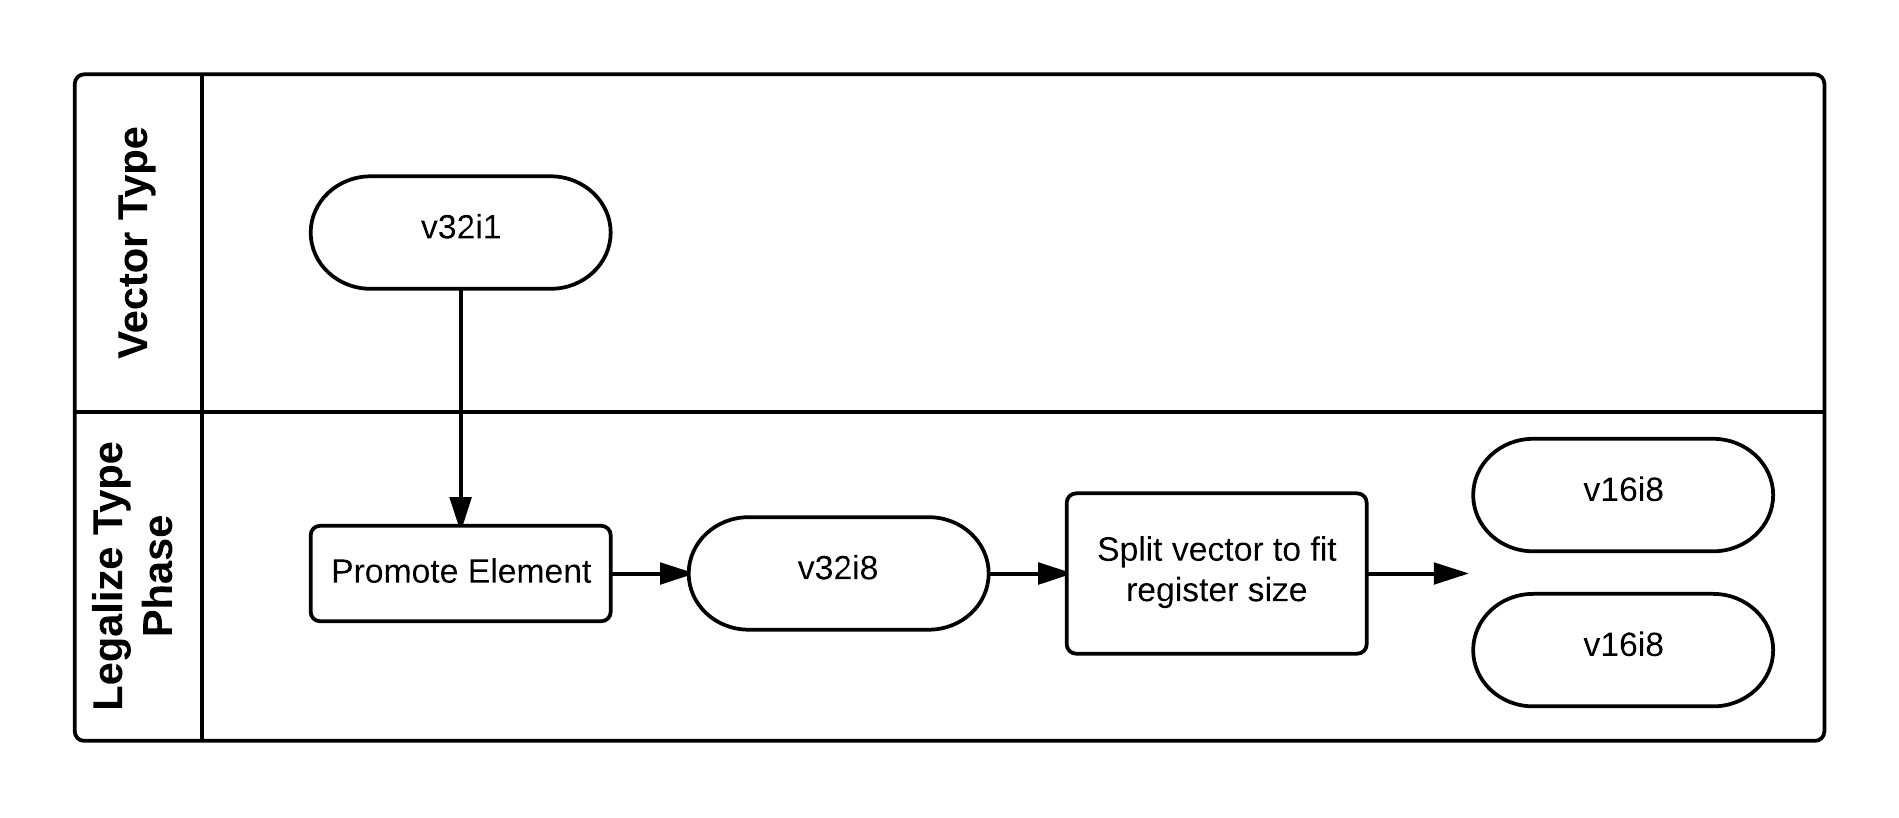
\includegraphics[width=140mm]{draw/v32i1_legalize_type.png}
  \caption{Type legalize process for $v32i1$ vector}
  \label{figure:v32i1_legalize_type}
\end{figure}

LLVM applies the same promote element strategy to vectors of $i2$ and $i4$, which would lead to huge selectionDAG generation and thus poor machine code. On the other hand, $i1$, $i2$ and $i4$ vectors are important to Parabix performance-critical operations, such as transposition and deletion; Parabix applications, such as DNA sequence (ATCG pairs) matching which can be encoded into $i2$ vectors most efficiently, requires a better support of small element vectors. All these reasons motivate us to find better implementation of $i1$, $i2$ and $i4$ vectors.

\section{LLVM Vector Legalization}
In LLVM IR, programmer can write any kind of vectors, even $v1024i3$, and those vectors may not be supported by the target machine. LLVM has the notion of a "legal" vs. "illegal". A type is legal for a target only if it is supported by some operation. In selectionDAG, a DAG node is legal only if the target supports the operation and operands type. For example, $v16i8$ is legal on X86 SSE2 architecture, since the architecture supports ADD on 2 $v16i8$ vectors; but it does not support multiplication on 2 $v16i8$ vectors, so that the DAG node MUL on $v16i8$ is illegal. LLVM has legalize types and legalize operations phases to turn illegal type or DAG into legal\cite{llvm_code_gen}.

Legalize type phase has three ways to legalize vector types\cite{hybrid_simd_type_legalize}: \textit{Scalarization}, \textit{Vector Widening} and \textit{Vector Element Promotion}.

\begin{itemize}
    \item \textbf{Scalarization} splits the vector into multiple scalars. It is often used for $v1iX$ as the edge case when LLVM is trying to split the incoming vector into sub vectors.
    \item \textbf{Vector Widening} adds dummy elements to make the vector fit the right register size. It will not change the type of the elements, e.g.\ $v4i8$ to $v16i8$.
    \item \textbf{Vector Element Promotion} preserves the number of elements, but promote the element type to a wider size, e.g.\ $v4i8$ to $v4i32$.
\end{itemize}

None of these strategies would legalize small element vectors properly. Think about $v32i1$, it fits in the general 32-bit registers, and we can not benefit from extending or splitting the vector in wider or more registers, not to mention scalarizing it. It would be the best to store $v32i1$ vectors just in the general 32-bit register and properly handle the operations on them.

After type legalization, we may still have illegal DAG node, such as multiplication on $v16i8$ for X86 SSE2 architecture; thus we need legalize operations phase. There are three strategies in this phase:

\begin{itemize}
    \item \textbf{Expansion}: Use another sequence of operations to emulate the operation. Expansion strategy is often general.
    \item \textbf{Promotion}: Promote the operand type to a larger type that support the operation.
    \item \textbf{Custom}: Write a target-specific code to implement the legalization. Similar to Expansion, but with a specific target in mind.
\end{itemize}

\section{Inplace Lowering Strategy}

Inspired by IDISA+\cite{hua_idisa}, we provide the fourth way to legalize vector type: Inplace Lowering. It is called "inplace" because we do not move the data around. A trivial example would be logical operations on \verb|<32 x i1>|; we can simply bitcast \verb|<32 x i1>| to \verb|i32| and perform the same operation. Almost all the operations on $vXi1$ can be simulated with logic operations on $iX$ (except INSERT VECTOR ELT and EXTRACT VECTOR ELT), as listed in table~\ref{table:vxi1}.

Inplace lowering strategy is implemented in the legalize operations phase since the legalizer is bounded to each specific operation. To make the operands type pass through the legalize types phase without being modified, we "type legalize" the vector of $i2^k$, and then handle the operation with such operands type all together. Figure~\ref{figure:v32i1_compare} gives an example of our vector legalization on $v32i1$ compared with LLVM default process.

\begin{figure}[ht!]
  \centering
  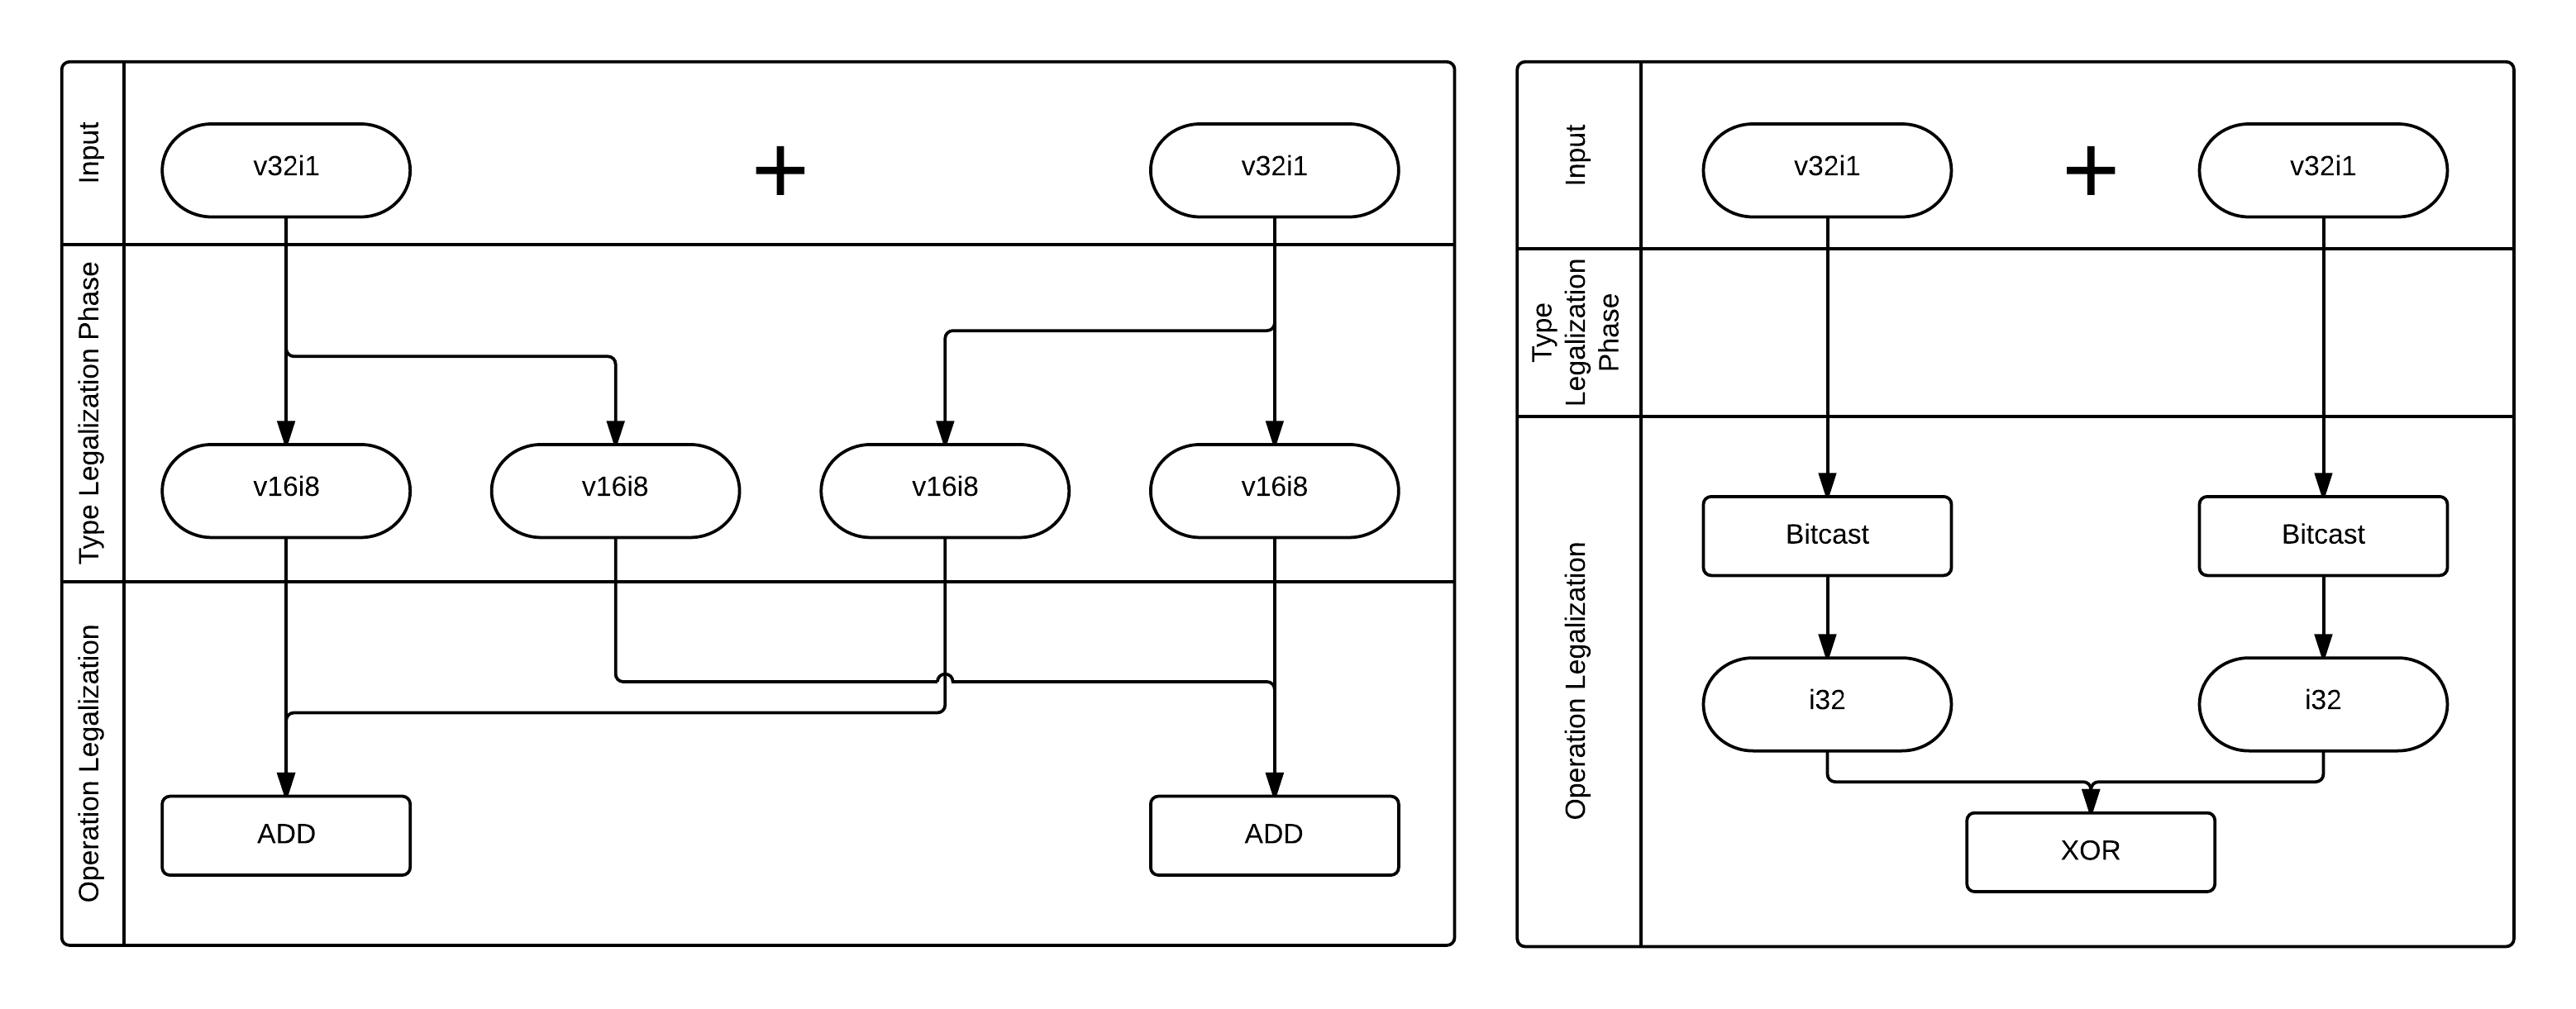
\includegraphics[width=150mm]{draw/v32i1_compare.png}
  \caption[Comparison between LLVM default legalize process and inplace lowering.]{Comparison between LLVM default legalize process (left) and inplace lowering (right). The right marks $v32i1$ type legal and handles the operation ADD in the legalize operations phase. This will keep the data in the general registers without being promoted or expanded.}
  \label{figure:v32i1_compare}
\end{figure}

\begin{table}
  \begin{center}
    \begin{tabular}{|l|l|}
      \hline
      Operation & Semantics                                                             \\ \hline
      NE        & Integer comparison between vectors. $c_i = 1$ if $a_i$ is not equal to $b_i$.    \\ \hline
      EQ        & $c_i = 1$ if $a_i$ is equal to $b_i$                                  \\ \hline
      LT        & $c_i = 1$ if $a_i < b_i$. $a_i$ and $b_i$ is viewed as signed integer \\ \hline
      GT        & $c_i = 1$ if $a_i > b_i$. $a_i$ and $b_i$ is viewed as signed integer \\ \hline
      ULT       & Same with LT, but numbers are viewed as unsigned integer              \\ \hline
      UGT       & Same with GT, but numbers are viewed as unsigned integer              \\ \hline
      SHL       & $c_i = a_i << b_i$. Element wise shift left                            \\ \hline
      SRL       & $c_i = a_i >> b_i$. Element wise logic shift right                     \\ \hline
      SRA       & $c_i = a_i >> b_i$. Element wise arithmetic shift right                \\ \hline
    \end{tabular}
  \end{center}
  \caption[Supported operations and its semantics.]{Supported operations and its semantics. $A, B$ is the operands, $C$ is the result. $a_i, b_i, c_i$ is the $i_{th}$ element.}
  \label{table:semantics}
\end{table}

\begin{table}
  \begin{center}
    \begin{tabular}{|c|c|}
      \hline
      Operation on $vXi1$ & $iX$ equivalence \\ \hline
      ADD(A, B) & XOR(A', B') \\ \hline
      SUB(A, B) & XOR(A', B') \\ \hline
      MUL(A, B) & AND(A', B') \\ \hline
      AND(A, B) & AND(A', B') \\ \hline
      OR(A, B) & OR(A', B') \\ \hline
      XOR(A, B) & XOR(A', B') \\ \hline
      NE(A, B) & XOR(A', B') \\ \hline
      EQ(A, B) & NOT(XOR(A', B')) \\\hline
      LT(A, B), UGT(A, B) & AND(A', NOT(B')) \\\hline
      GT(A, B), ULT(A, B) & AND(B', NOT(A')) \\\hline
      SHL(A, B), SRL(A, B) & AND(A', NOT(B')) \\\hline
      SRA(A, B) & A' \\\hline
    \end{tabular}
  \end{center}
\caption[Legalize operations on $vXi1$ with $iX$ equivalence.]{Legalize operations on $vXi1$ with $iX$ equivalence. A, B are $vXi1$ vectors, A', B' are $iX$ bitcasted from $vXi1$. For $v128i1$, we use $v2i64$ instead of $i128$ since LLVM supports the former better.}
\label{table:vxi1}
\end{table}

\subsection{Lowering for $vXi2$}
Vector type $vXi2$ has important role in Parabix transposition and inverse transposition. Ideal Three-Stage Parallel Transposition\cite{transposition} requires \verb|hsimd<4>::packh| and \verb|hsimd<4>::packl|, which can be implemented with shufflevectors on $v64i2$. Shufflevectors of $v64i2$ are also required by Ideal Inverse Transposition, for \verb|esimd<2>::mergeh| and \verb|esimd<2>::mergel|. Transposition is the first step of every parabix application\cite{inductive_doubling_principle} and it is the principle overhead for some application like regular expression matching\cite{rob_regex}. So good code generation for $vXi2$ is important.

Lowering $vXi2$ is harder than $vXi1$, so we propose a systematic framework using logic and 1-bit shifting operations. Consider $A, B$ as two $i2$ integers, $A=a_0a_1$ and $B=b_0b_1$, we can construct a truth table for every operation $C = OP(A, B)$. We then calculate the first bit and the second bit of $C$ separately with the logic combinations of $a_0, a_1, b_0, b_1$ and turn this into \textit{Circuit Minimization Problem}: find minimized boolean functions for $c_0$ and $c_1$. We use Quine-McCluskey algorithm\cite{johnson1981quine} to solve it; an example can be found in Table~\ref{table:quine}.

\begin{table}[h]
  \centering
  \begin{tabular}{ccc}
    \hline
    A                   & B                   & C                  \\ \hline
    00                  & 00                  & 00                 \\
    00                  & 01                  & 01                 \\
    00                  & 10                  & 10                 \\
    \multicolumn{3}{c}{$\ldots$}                                        \\
    11                  & 11                  & 10                 \\ \hline
  \end{tabular}

  \begin{tabular}{lll}
    \\
    \multicolumn{3}{c}{$c_0 = (a_0 \oplus b_0) \oplus (a_1 \land b_1)$} \\
    \multicolumn{3}{c}{$c_1 = a_1 \oplus b_1$}
  \end{tabular}
  \caption{Truth table of ADD on 2-bit integers and the minimized boolean functions for $C$.}
  \label{table:quine}
\end{table}

Once we get the minimized boolean functions, we can apply it onto the whole $vXi2$ vector. Let us introduce one operation first, {\tt IFH1}. {\tt IFH1(Mask, A, B)} selects bits from vector {\tt A} and {\tt B} according to the {\tt Mask}. If the $i_{th}$ bit of {\tt Mask} is $1$, $\text{\tt A}_i$ is selected, otherwise $\text{\tt B}_i$ is selected. {\tt IFH1(Mask, A, B)} simply equals to $(\text{\tt Mask} \land \text{\tt A}) \lor (\lnot \text{\tt Mask} \land \text{\tt B})$.

Then if we have calculated the all high bits ($c_0$ for all the element) and low bits ($c_1$ for all the element), we can combine them with {\tt IFH1} with special {\tt HiMask}, which equals to $101010 \ldots 10$, 128 bits long in binary. To calculate all the high bits of each $i2$ element, we bitcast A, B into full register type (e.g.\ $v32i1$ to $i32$, $v64i2$ to $i128$ or $v2i64$) and then do the following substitution on the minimized boolean functions:

\begin{itemize}
    \item For $a_0$ and $b_0$, replace it with $A$ and $B$.
    \item For $a_1$ and $b_1$, replace it with $A << 1$ and $B << 1$.
    \item Keep all the logic operations.
\end{itemize}

So $c_0 = (a_0 \oplus b_0) \oplus (a_1 \land b_1)$ becomes $(A \oplus B) \oplus ((A << 1) \land (B << 1))$, which simplifies to $(A \oplus B) \oplus ((A \land B) << 1)$. We use shifting to move every $a_1$ and $b_1$ in place. For all the lower bits of each $i2$ element, the rules are similar:

\begin{itemize}
    \item For $a_1$ and $b_1$, replace it with $A$ and $B$.
    \item For $a_0$ and $b_0$, replace it with $A >> 1$ and $B >> 1$.
    \item Keep all the logic operations.
\end{itemize}

Program~\ref{program:genloweradd} is the actual custom code to lower $v64i2$ addition. One thing to mention here is that we deploy a template system to automatically generate custom lowering code and the corresponding testing code. We would describe the template system later in Chapter~\ref{five}.

\begin{program}
\begin{verbatim}
static SDValue GENLowerADD(SDValue Op, SelectionDAG &DAG) {
  MVT VT = Op.getSimpleValueType();
  MVT FullVT = getFullRegisterType(VT);
  SDNodeTreeBuilder b(Op, &DAG);

  if (VT == MVT::v64i2) {
    SDValue A = b.BITCAST(Op.getOperand(0), FullVT);
    SDValue B = b.BITCAST(Op.getOperand(1), FullVT);

    return b.IFH1(/* 10101010...10, totally 128 bits */
                  b.HiMask(128, 2),
                  /* C0 = (A0 ^ B0) ^ (A1 & B1) */
                  b.XOR(b.XOR(A, B), b.SHL<1>(b.AND(A, B))),
                  /* C1 = (A1 ^ B1)*/
                  b.XOR(A, B));
  }

  llvm_unreachable("GENLower of add is misused.");
  return SDValue();
}
\end{verbatim}
\caption{The function generated to lower ADD on $v64i2$.}
\label{program:genloweradd}
\end{program}

\subsection{Inductive Doubling Principle}
Now we have better code generation for $vXi1$ and $vXi2$, $vXi4$ vectors are our next optimization target. Shufflevectors of $vXi4$ are used in \verb|hsimd<8>::packh|, \verb|hsimd<8>::packl| and \verb|esimd<4>::mergeh|, which are required by Ideal Three-Stage Transposition / Inverse Transposition. But unfortunately, the strategies discussed above cannot be applied to $vXi4$ efficiently.

Circuit Minimization Problem is NP-hard\cite{wiki_quine, kabanets2000circuit}. For $vXi4$, we would have 4 boolean functions of 8 variables: $c_i = f_i(a_0, a_1, a_2, a_3, b_0, b_1, b_2, b_3), i \in \left\{{0, 1, 2, 3}\right\}$, and it is known that most boolean functions on $n$ variables have circuit complexity at least $2^n/n$\cite{kabanets2000circuit} and we need 1-bit, 2-bit, 3-bit shifting on $A$, $B$. So the framework on $vXi2$ could not generate efficient code for us at this time. Instead, we introduce \textit{Inductive Doubling Principle} \cite{inductive_doubling_principle} and we will show that this general principle can be applied for $vXi4$ and even wider vector element type, e.g.\ multiplication on $v16i8$, to get better performance.

\begin{figure}[ht!]
\centering
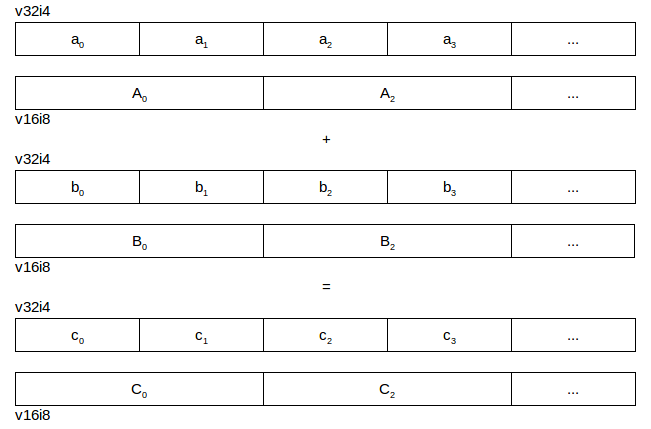
\includegraphics[width=110mm]{draw/add_4.png}
\caption[Addition of two $v32i4$ vectors.]{To add 2 $v32i4$ vectors, $a$ and $b$, we bitcast them into $v16i8$ vectors. The lower 4 bits of $A_0 + B_0$ gives us $c_1$. We then mask out $a_1$ and $b_1$ (set them to zero), do add again, and the higher 4 bits of the sum is $c_0$.}
\label{figure:add_4}
\end{figure}

\begin{figure}[ht!]
\centering
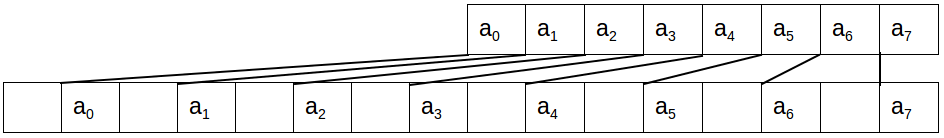
\includegraphics[width=130mm]{draw/v8i4_v8i8.png}
\caption[LLVM default type legalization of $v8i4$ to $v8i8$.]{LLVM default type legalization of $v8i4$ to $v8i8$. $a_0$ to $a_7$ are $i4$ elements and they are shifted with different offsets during the element type promotion.}
\label{figure:v8i4_v8i8}
\end{figure}

We use $v32i4$ as an example to illustrate Inductive Doubling Principle. To legalize $v32i4$, LLVM would promote this type into $v32i8$, widen every element to $i8$ and shift every element except the first one. Figure~\ref{figure:v8i4_v8i8} shows an example of widening $v8i4$ into $v8i8$, we can see unnecessary movement of vector element during widening. On a platform with 128 bits SIMD register, $v32i8$ will further be divided into two $v16i8$ and take 2 registers to hold, while the original type $v32i4$ has 128 bits in size and should be able to reside in only 1 register. Inductive Doubling Principle could achieve the latter for us. It would bitcast the vector inplace, view the same register as $v16i8$ type and emulate $i4$ operations with $i8$; e.g.\ in Figure~\ref{figure:add_4}, to get \verb|add <32 x i4> %a, %b|, we calculate $c_0, c_2, \ldots, c_{30}$ (high 4 bits in each $i8$ element) and $c_1, c_3, \ldots, c_{31}$ (low 4 bits in each $i8$ element) separately with 2 $v16i8$ additions:

\begin{gather}
C = IFH1(HiMask_8, A \land HiMask_8 + B \land HiMask_8, A + B) \\
HiMask_8 = (1111000011110000 \ldots 11110000)_2
\end{gather}

Generally, as Dr Cameron wrote, "inductive doubling refers to a general property of certain kinds of algorithm that systematically double the values of field widths or other data attributes with each iteration."\cite{inductive_doubling_principle}. He described four key elements of this architecture:
\begin{itemize}
    \item A core set of binary functions on $iX$ vectors, for all $X = 2^k$. To work with parallel bit streams, the operation ADD, SUB, SHL, SRL and ROTL (rotate left) comprise the set.
    \item A set of \textit{half-operand modifiers} that make possible the inductive processing of $i2X$ in terms of combinations of $iX$. These modifiers select either the lower $X$ bits of each $i2X$ element or the higher $X$ bits.
    \item Packing operations that compress two {\tt <N x iX>} vectors into one {\tt <2N x i(X/2)>} vector. Like {\tt hsimd<8>::packh} we mentioned in Chapter~\ref{three}.
    \item Merging operations that produce one {\tt <N x iX>} vector from two {\tt <2N x i(X/2)>} vectors. Like {\tt esimd<8>::mergeh}, it is the reverse function of packing.
\end{itemize}

For this section, we will only use the fact that we can emulate SIMD operations on $iX$ vectors with $iX/2$ or $i2X$ vector operations. We implemented all the operations on $vXi4$ with this principle and the algorithm is listed in Table~\ref{table:vXi4}. One thing needs explain is SETCC, which is the internal representation of integer comparison in LLVM\@. It has a third operand to determine comparison type, such as SETEQ (equal), SETLT (signed less than), and SETUGE (unsigned greater or equal to). The third operand preserves in our algorithm.

\begin{table}[h]
\centering
\begin{tabular}{ccc}
\multicolumn{3}{c}{$C = IFH1(HiMask_8, HiBits, LowBits)$} \\ \hline
\multicolumn{1}{|c|}{\multirow{2}{*}{\begin{tabular}[c]{@{}c@{}}Operation\\ $v32i4$\end{tabular}}} & \multicolumn{1}{c|}{$HiBits$} & \multicolumn{1}{c|}{$LowBits$} \\ \cline{2-3}
\multicolumn{1}{|c|}{} & \multicolumn{2}{c|}{All operation is on $v16i8$} \\ \hline
\multicolumn{1}{|c|}{MUL} & \multicolumn{1}{c|}{$MUL(A >> 4, B >>4) << 4$} & \multicolumn{1}{c|}{Default} \\ \hline
\multicolumn{1}{|c|}{SHL} & \multicolumn{1}{c|}{$SHL(A \land HiMask_8, B >>4)$} & \multicolumn{1}{c|}{$SHL(A, B \land LowMask_8)$} \\ \hline
\multicolumn{1}{|c|}{SRL} & \multicolumn{1}{c|}{$SRL(A, B>>4)$} & \multicolumn{1}{c|}{$SRL(A \land LowMask_8, B \land LowMask_8)$} \\ \hline
\multicolumn{1}{|c|}{SRA} & \multicolumn{1}{c|}{$SRA(A, B>>4)$} & \multicolumn{1}{c|}{$SRA(A << 4, (B \land LowMask_8)) >> 4$} \\ \hline
\multicolumn{1}{|c|}{SETCC} & \multicolumn{1}{c|}{Default} & \multicolumn{1}{c|}{$SETCC(A << 4, B << 4)$} \\ \hline
\multicolumn{1}{|c|}{Default OP} & \multicolumn{1}{c|}{$OP(A \land HiMask_8, B \land HiMask_8)$} & \multicolumn{1}{c|}{$OP(A, B)$} \\ \hline
\multicolumn{1}{l}{In the table:} & \multicolumn{1}{l}{} & \multicolumn{1}{l}{} \\
 & \multicolumn{2}{l}{$A >> 4$: logic shift right every $i8$ element by 4 bits} \\
 & \multicolumn{2}{l}{$A << 4$: shift left of every $i8$ element by 4 bits} \\
\multicolumn{1}{l}{} & \multicolumn{2}{l}{$HiMask_8 = (11110000 \ldots 11110000)_2$} \\
\multicolumn{1}{l}{} & \multicolumn{2}{l}{$LowMask_8 = (00001111 \ldots 00001111)_2$}
\end{tabular}
\caption[Algorithm to lower $v32i4$ operations.]{Algorithm to lower $v32i4$ operations. The legalization input is $c = OP(a, b)$, where $a, b, c$ are $v32i4$ vectors. $A, B, C$ is the bitcasted results from $a, b, c$ and they are all $v16i8$ type.}
\label{table:vXi4}
\end{table}

Furthermore, this method is applicable to vectors of wider element type. Multiplication on $v16i8$, for example, generates poor code on LLVM 3.4 (Program~\ref{program:mult_8}): the vectors are finally scalarized and 16 multiplications on $i8$ elements are generated. With inplace promotion, we bitcast the operands into $v8i16$ and generates 2 SIMD multiplications ($pmullw$) instead.

\begin{program}
\begin{verbatim}
define <16 x i8> @mult_8(<16 x i8> %a, <16 x i8> %b) {
entry:
  %c = mul <16 x i8> %a, %b
  ret <16 x i8> %c
}
\end{verbatim}
\begin{multicols}{2}
\begin{verbatim}
# LLVM 3.4 default:
  pextrb▸ $1, %xmm0, %eax
  pextrb▸ $1, %xmm1, %ecx

  mulb▸   %cl
  movzbl▸ %al, %ecx
  pextrb▸ $0, %xmm0, %eax
  pextrb▸ $0, %xmm1, %edx

  mulb▸   %dl
  movzbl▸ %al, %eax
  movd▸   %eax, %xmm2
  pinsrb▸ $1, %ecx, %xmm2
  pextrb▸ $2, %xmm0, %eax
  pextrb▸ $2, %xmm1, %ecx

  mulb▸   %cl
  movzbl▸ %al, %eax
  pinsrb▸ $2, %eax, %xmm2
  pextrb▸ $3, %xmm0, %eax
  pextrb▸ $3, %xmm1, %ecx

  mulb▸   %cl
  movzbl▸ %al, %eax
  pinsrb▸ $3, %eax, %xmm2
  pextrb▸ $4, %xmm0, %eax
  pextrb▸ $4, %xmm1, %ecx
  ...
  ...
  (16 mulb blocks in total)
\end{verbatim}
\columnbreak
\begin{verbatim}
# Inductive doubling result:
  movdqa▸ %xmm0, %xmm2
  pmullw▸ %xmm1, %xmm2
  movdqa▸ .LCPI0_0(%rip), %xmm3
  movdqa▸ %xmm3, %xmm4
  pandn▸  %xmm2, %xmm4
  psrlw▸  $8, %xmm1
  psrlw▸  $8, %xmm0
  pmullw▸ %xmm1, %xmm0
  psllw▸  $8, %xmm0
  pand▸   %xmm3, %xmm0
  por▸    %xmm4, %xmm0
  retq
\end{verbatim}
\end{multicols}
\caption[Inductive doubling principle on $v16i8$ multiplication.]{Inductive doubling principle on $v16i8$ multiplication. LLVM 3.4 generate poor machine code, which will $pextrb$ every $i8$ field and multiply them with $mulb$. We simplify it through 2 $pmullw$, which is the multiplication on $v8i16$.}
\label{program:mult_8}
\end{program}

However, the algorithm in Table~\ref{table:vXi4} cannot guarantee the best performance. Addition on $v32i4$ requires 2 $v16i8$ additions, but we can actually implement it with one. Look back to Figure~\ref{figure:add_4}, we need to mask out $a_1$, $b_1$ and do add again, because $a_1 + b_1$ may produce carry bit to the high 4 bits. If we mask out only the high bit of $a_1$ and $b_1$, still we will not produce carry and we can calculate $c_0$ and $c_1$ together in one $v16i8$ addition. All we need to solve is how to put the high bit back. The following equations describe the 1-add algorithm:

\begin{gather}
  m = (10001000 \ldots 1000)_2 \\
  A_h = m \land A \\
  B_h = m \land B \\
  z = (A \land \lnot A_h) + (B \land \lnot B_h) \label{eq:1_add_z}\\
  r = r \oplus A_h \oplus B_h \label{eq:1_add_r}
\end{gather}

Equation~\eqref{eq:1_add_z} uses only one $v16i8$ addition and equation~\eqref{eq:1_add_r} put the high bit back. Our vector legalization framework is flexible enough that we can choose to legalize $v32i4$ addition with 1-add algorithm while keeping the rest $v32i4$ operations under general inplace promotion strategy. We will discuss our framework implementation in Chapter~\ref{five}.

\section{LLVM Vector Operation of $i2^k$}
In addition to the binary operations listed in Table~\ref{table:semantics}, LLVM provides convenient vector operations like \textit{insertelement}, \textit{extractelement} and \textit{shufflevector}, internally, they are DAG node INSERT VECTOR ELT, EXTRACT VECTOR ELT and VECTOR SHUFFLE\@. Another important internal node is BUILD VECTOR\@. In this section, we will discuss how to custom lower these nodes on $i2^k$ vectors.

BUILD VECTOR takes an array of scalars as input and output a vector with these scalars as elements. Take $v64i2$ vector on X86 SSE2 architecture for an example; ideally, the input would provide an array of 64 $i2$ scalars and BUILD VECTOR assembles them into a $v64i2$ vector. More specifically, since $i2$ is illegal on all X86 architecture, the legal input is actually 64 $i8$ scalars. The naive approach would be creating an "empty" $v64i2$ vector, truncating every $i8$ into $i2$ and inserting it into the proper location of the "empty" vector. We propose a better approach by rearranging the index.

Let us denote the input array as $a_0, a_1, \ldots, a_{63}$, $a_i$ is all $i8$. We rearrange them according to Table~\ref{table:build_vector} and build 4 $v16i8$ vectors $V_1, V_2, V_3, V_4$. The final build result is:
\begin{equation}
  V = V_1 \lor (V_2 << 2) \lor (V_3 << 4) \lor (V_4 << 6)
\end{equation}

\begin{table}[h]
\centering
\begin{tabular}{|p{1cm}|p{1cm}|p{1cm}|p{1cm}|p{1cm}|p{1cm}|r}
\cline{1-6}
$a_{60}$ & $\ldots$ & $a_{12}$ & $a_8$ & $a_4$ & $a_0$ & $V_1$ \\ \cline{1-6}
$a_{61}$ & $\ldots$ & $a_{13}$ & $a_9$ & $a_5$ & $a_1$ & $V_2$ \\ \cline{1-6}
$a_{62}$ & $\ldots$ & $a_{14}$ & $a_{10}$ & $a_6$ & $a_2$ & $V_3$ \\ \cline{1-6}
$a_{63}$ & $\ldots$ & $a_{15}$ & $a_{11}$ & $a_7$ & $a_3$ & $V_4$ \\ \cline{1-6}
\end{tabular}
\caption{Rearranging index for BUILD VECTOR on $v64i2$}
\label{table:build_vector}
\end{table}

SIMD OR and SHL are used in this formula, thus improving the performance by parallel computing. Rearranging index approach can be easily generalized to fit BUILD VECTOR of $v128i1$ and $v32i4$.

EXTRACT VECTOR ELT takes 2 operands, a vector $V$ and an index $i$. It returns the $i_{th}$ element of $V$. The semantics would not allow much parallelism in the implementation. On X86 architecture, there are built-in intrinsics to extract vector element, such as $pextrb$ ($i8$), $pextrw$ ($i16$), $pextrd$ ($i32$) and $pextrq$ ($i64$); for smaller element type, we could extract the wider integer that contains it, shift the small element to the lowest bits and truncate. Following algorithm gives an example of extracting the $i_{th}$ element from the $v64i2$ vector {\tt V}.

\begin{itemize}
  \item Bitcast {\tt V} to $v4i32$ {\tt V'} and extract the proper $i32$ {\tt E}. Since every $i32$ contains 16 $i2$ elements, the index of {\tt E} is $\lfloor i / 16 \rfloor$.
  \[\text{\tt V'} = \text{\tt bitcast <64 x i2> V to <4 x i32>} \]
  \[\text{\tt E} = \text{\tt extract element V',} \lfloor i / 16 \rfloor \]
  \item Shift right {\tt E}, to put the element we want in the lowest bits.
  \[\text{\tt E'} = \text{\tt E >>} (2 \times (i \bmod 16))\]
  \item Truncate the high bits of {\tt E'} to get the result.
  \[\text{\tt R} = \text{\tt truncate i32 E' to i2}\]
\end{itemize}

The choice of $v4i32$ does not make a difference, we can use any of the wider element vector type mentioned above. On the X86 architecture, the support of extraction on $v8i16$ starts at SSE2, while others start at SSE4.1, so we choose $v8i16$ extraction in our code to target broader range of machines.

INSERT VECTOR ELT is similar, it takes 3 operands, a vector $V$, an index $i$ and an element $e$. It inserts $e$ into the $i_{th}$ element of $V$ and returns the new vector. Same as EXTRACT VECTOR ELT, X86 SSE2 supports $v8i16$ insertion ($pinsrw$), SSE4.1 supports $v16i8$ ($pinsrb$), $v4i32$ ($pinsrd$) and $v2i64$ ($pinsrq$); for smaller element type, we could extract the wider integer that contains the element, modify the integer and insert it back. Following algorithm gives an example of inserting {\tt e} into the $i_{th}$ element of the $v64i2$ vector {\tt V}.

\begin{itemize}
  \item Bitcast {\tt V} to $v4i32$ {\tt V'} and extract the proper $i32$ {\tt E}.
  \[\text{\tt V'} = \text{\tt bitcast <64 x i2> V to <4 x i32>} \]
  \[\text{\tt E} = \text{\tt extract element V',} \lfloor i / 16 \rfloor \]

  \item Truncate {\tt e} and shift it to the correct position.
  \[\text{\tt e'} = \text{\tt zero extend (e} \land (11)_2 \text{\tt ) to i32} \]
  \[\text{\tt f} = \text{\tt e' <<} (2 \times (i \bmod 16))\]

  \item Mask out old content in {\tt E}, put in the new element.
  \[\text{\tt m} = (11)_2 << (2 \times (i \bmod 16)) \]
  \[\text{\tt E'} = (\text{\tt E} \land \lnot \text{\tt m}) \lor \text{\tt f}\]

  \item Insert back {\tt E'} to generate the new vector {\tt R}.
  \[\text{\tt R} = \text{\tt insert element V', E',} \lfloor i / 16 \rfloor \]
\end{itemize}

We have discussed VECTOR SHUFFLE in Chapter~\ref{three}. We did not develop a general lowering strategy for the small element VECTOR SHUFFLE\@. In stead, we focused more on special cases that matter to Parabix critical operations, we optimized those cases to match performance of the hand-written library.

\section{Long Stream Addition}
Parabix technology has the concept of adding 2 unbounded streams and of course this needs to be translated into an block-at-a-time implementation\cite{rob_regex}. One important operation is unsigned addition of 2 SIMD registers with carry-in and carry-out bit e.g.\ \verb|add i128 %a, %b| or \verb|add i256 %a, %b| with $i1$ carry-in bit \verb:c_in: and generates $i1$ carry-out bit \verb:c_out:. Dr Cameron developed a general model using SIMD methods for efficient long-stream addition up to 4096 bits in \cite{rob_regex}.

In this section, we will replace the internal logic of wide integer addition ($i128$, $i256$ etc. ) of LLVM with the Parabix long-stream addition. Same with Dr Cameron's work in \cite{rob_regex}, we assume the following SIMD operations on $i64$ vectors legal on the target:
\begin{itemize}
    \item \verb|add <N x i64> X, Y|, where $\text{\tt N} = RegisterSize / 64$. SIMD addition on each corresponding element of the $i64$ vectors, no carry bits could cross the element boundary.
    \item \verb|icmp eq <N x i64> X, -1|: compare each element of {\tt X} with the all-one constant, returning an \verb|<N x i1>| result.
    \item \verb|signmask <N x i64> X|: collect all the sign bit of $i64$ elements into a compressed \verb|<N x i1>| vector. From the LLVM speculation, this operation is equivalent to \verb|icmp lt <N x i64> X, 0|, which is the signed less-than comparison of each $i64$ element with 0. In the real implementation we use target-specific operations for speed, e.g. $movmsk\_pd$ for SSE2 and $movmsk\_pd\_256$ for AVX.
    \item Normal bitwise logic operations on \verb|<N x i1>| vectors. For small {\tt N}, native support may not exist, so we bitcast \verb|<N x i1>| to $iN$ and then zero extend it to $i32$. This conversion could also help with the 1-bit shift we use later.
    \item \verb|zext <N x i1> m to <N x i64>|: this corresponds to \verb|simd<64>::spread(X)| in \cite{rob_regex}, which would distribute the {\tt N} bits of the mask, one bit each to the lower end of the {\tt N} $i64$ elements.
\end{itemize}

We then present the long stream addition of 2 $N \times 64$ bit values {\tt X} and {\tt Y} with these operations as the following.
\begin{enumerate}
    \item Get the vector sums of {\tt X} and {\tt Y}.
    \[\text{\tt R} = \text{\tt add <N x i64> X, Y} \]
    \item Get sign masks of {\tt X}, {\tt Y} and {\tt R}.
    \[\text{\tt x} = \text{\tt signmask <N x i64> X} \]
    \[\text{\tt y} = \text{\tt signmask <N x i64> Y} \]
    \[\text{\tt r} = \text{\tt signmask <N x i64> R} \]
    \item Compute the carry mask {\tt c}, bubble mask {\tt b} and the increment mask {\tt i}.
    \[\text{\tt c} = (\text{\tt x} \wedge \text{\tt y}) \vee ((\text{\tt x} \vee \text{\tt y}) \wedge \neg \text{\tt r})\]
    \[\text{\tt b} = \text{\tt icmp eq <N x i64> R, -1}\]
    \[\text{\tt i} = \text{\tt MatchStar(c*2+c\_in, b)}\]
    MatchStar is a key Parabix operation which is developed for regular expression matching:
    \[\text{\tt MatchStar}(M, C) = (((M \wedge C) + C)  \oplus C) | M\]
    \item Compute the final result {\tt Z} and carry-out bit {\tt c\_out}.
    \[\text{\tt S} = \text{\tt zext <N x i1> i to <N x i64>}\]
    \[\text{\tt Z} = \text{\tt add <N x i64> R, S}\]
    \[\text{\tt c\_out} = \text{\tt i >> N}\]
    One note here for the mask type: {\tt c} and {\tt i} are literally all \verb|<N x i1>| vectors, but we actually bitcast and zero extend them into $i32$. This is useful in the formula {\tt c*2+c\_in}, {\tt MatchStart} and {\tt i >> N}; in fact, after we shift left {\tt c} by {\tt c*2}, we already have an $N+1$ bit integer which will not fit in \verb|<N x i1>| vector. The same is true for {\tt i}; so when we write {\tt zext <N x i1> i to <N x i64>}, there is an implicit truncating to get the lower {\tt N} bits of {\tt i}, but when we shift right {\tt i} by {\tt i >> N}, we do not do such truncation.
\end{enumerate}

LLVM internally implement long integer addition with a sequence of ADDC and ADDE, which is just chained 64-bit additions (or 32-bit additions on 32-bit target). We replace that with the long stream addition model thus improving the performance by parallel computing. As the hardware evolves, wider SIMD registers would be introduced, like 512-bit register in Intel AVX512, our general implementation could easily adopt this change in hardware and add two $i512$ in constant time.

%%%%%%%%%%%%%%%%%%%%%%%%%%%%%%%%%%%%%%%%%%%%%%%%%
%
%     Chapter 5
%
%%%%%%%%%%%%%%%%%%%%%%%%%%%%%%%%%%%%%%%%%%%%%%%%

\chapter{Implementation}
\label{five}

In this Chapter, we describe our realization of Parabix technology inside the LLVM facility. LLVM is a well-structured open source compiler tool chain which is under rapid development. So during our implementation, we tried our best to follow its design principles while keeping our code modularized and isolated to be able to easily integrate with new versions of LLVM\@. Our goal of code design is to:
\begin{enumerate}
  \item Use general strategies across different types and operations to reduce repeated logic.
  \item Minimize code injection in the existing source and put Parabix logic in a separate module.
  \item Check correctness of every operation we implement. Since most of the test code follows the same pattern, they should be generated automatically to reduce repeated human work.
\end{enumerate}

Most of our code reside in LLVM Target-Independent Code Generator\cite{llvm_code_gen}. From Chapter~\ref{four}, we know that the current type legalization process of LLVM has a big performance penalty for small element vectors. So our approach marks $i1$, $i2$ and $i4$ vector legal type first, and then handles them in the operation legalization phase. For convenience, we name this set of vector types the \textit{Parabix Vector}.

We walk through the following steps to mark a type legal on a certain target:
\begin{itemize}
  \item \textbf{Add new register class in target description file.} LLVM uses TableGen (.td files) to describe target information which allows the use of domain-specific abstractions to reduce repetition \cite{llvm_code_gen}. Registers are grouped into register classes which further tie to a set of types. We introduced GR32X for 32-bit general register like EAX EBX for $v32i1$, GR64X for 64-bit general register like RAX RBX for $v64i1$, VR128PX for 128-bit vector register like XMM0 to XMM15 for $v128i1$, $v64i2$, $v32i4$  Types within the same register class can be bitcasted from one to the other, since they can actually reside in the same register.

  \item \textbf{Set calling convention.} They are two kinds of calling convention to set: return value and argument calling convention. For example, we instruct LLVM to assign $v64i2$ type return value to XMM0 to XMM3 registers, assign $v64i2$ argument type to XMM0 to XMM3 registers if SSE2 is available or to 16-byte stack slots otherwise.
\end{itemize}

Now the type legalization phase recognizes our $i1$, $i2$, $i4$ vectors as legal and passes them onto the operation legalization phase. We have two major methods to handle $i2^k$ vectors: \textit{Custom Lowering} and \textit{DAG Combining}.

\begin{figure}[ht!]
\centering
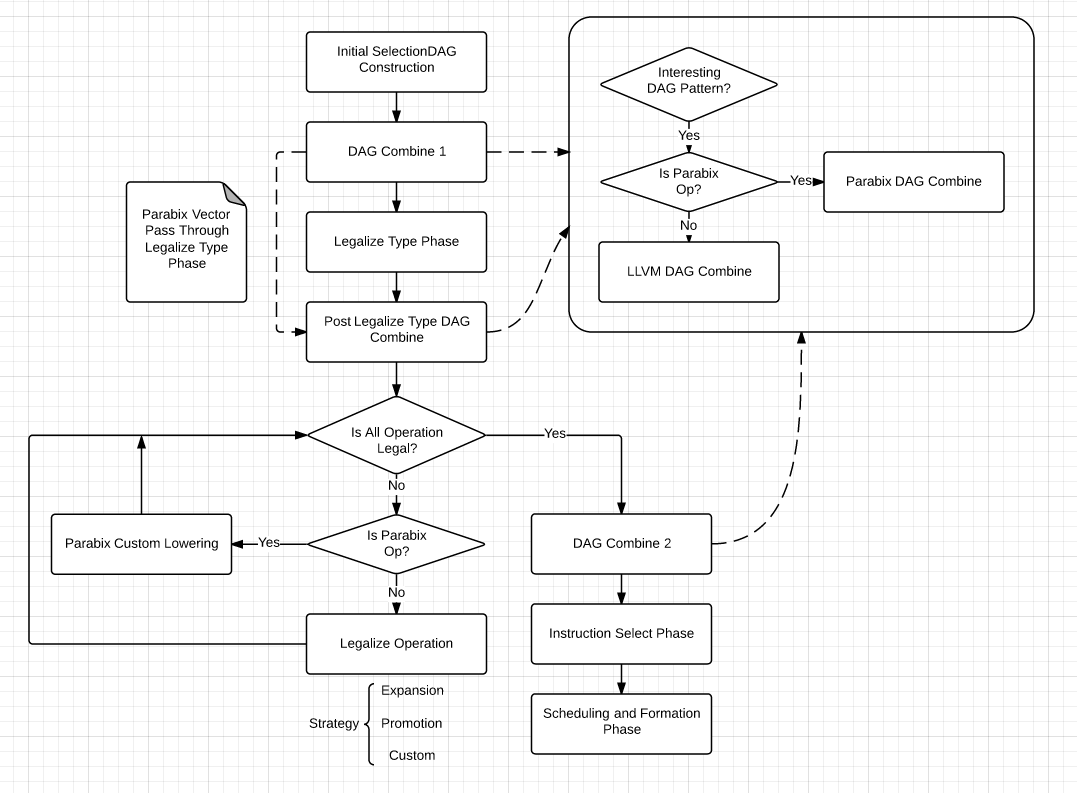
\includegraphics[width=140mm]{draw/system.png}
\caption[System overview: modified instruction selection process]{Overview of the modified instruction selection process. Logic for Parabix vectors are hooked into two places: the operation legalization phase and DAG Combine Phases. They are coloured with grey background.}
\label{figure:system}
\end{figure}

Figure~\ref{figure:system} gives an overview of our implementation. LLVM constructs a SelectionDAG with the input IR source code and then puts it through DAG Combine 1 for cleaning up and optimization. The optimized DAG is fed into the type legalization phase. We mark the Parabix Vectors type-legal so that they could pass through this phase without being changed. There is another DAG combining phase after the type legalization. Then, the resulting DAG is fed into the operation legalization phase which is done by iteration. Custom Lowering for Parabix resides in this phase. In each iteration, the legalizer checks every DAG node for its legality. If the node is illegal and performs operation on some Parabix vector, the Parabix Custom Lowering code will be called to legalize this node; otherwise the default LLVM logic will handle this illegal node. The iteration terminates when every DAG node is legal. Through iteration, the legalizer could introduce new illegal nodes into the graph.

After the operation legalization phase, there is another DAG combining to clean up the messy output. The last two steps for machine code generation remain the same. There is Parabix DAG Combine logic in all the three DAG combining phases. Each DAG combining phase maintains a work list. It traverses the DAG graph for specific operations. If the operation works with Parabix vectors and it fits a certain pattern, the Parabix DAG Combine logic will replace the node with a new node or a new sub-tree of nodes. Examples of DAG patterns can be found in Section~\ref{sec:long_shift}. Part(or all) of the new nodes can be appended to the work list so that the legalizer knows to combine it further later. There is no built-in iteration for DAG combining, but the iteration can be emulated by keeping appending the processed nodes to the work list if necessary.

In the following sections, we discuss some custom lowering strategies and how they are organized to fit our design goal. Then we give some examples of the Parabix DAG Combiner which are usually special cases for a certain operation. Finally we show how we use templates to generate code and test cases for the sake of DRY (don't repeat yourself).

\section{Standard Method For Custom Lowering}
\subsection{Custom Lowering Strategies}
After the type legalization phase, one shall not generate illegal types again. This means all the phases after type legalization are target-specific. But in practice, almost all the targets support $i8$, $i32$ and $i64$, so there are still general strategies we can apply across targets. For different types like $v32i1$ and $v128i1$, general strategies also exist to lower both of them. We define three legalize actions as the following:
\begin{enumerate}
    \item Bitcast to full register and replace the operation code. This is useful for all $i1$ vectors, we need to specify the new operation code when defining the action, e.g.\ XOR for ADD on $v32i1$.
    \item In-place promotion. Automatically apply $i2X$ vector operations on an $iX$ vector following the Inductive Doubling Principle.
    \item Custom. Same concept with LLVM Custom Lowering, manually replace an illegal DAG node with a sequence of new DAG nodes. They can be illegal nodes, but they cannot introduce illegal types. All $i2$ vectors are lowered here, also the 1-add version of the $v32i4$ addition.
\end{enumerate}

\subsection{DAG Combiner}
\label{sec:long_shift}
DAG Combiner is the supplement to the custom lowering facility. It often focuses on special cases e.g.\ one operation and a subset of possible operands. We give a few examples of Parabix DAG Combiner here.

\begin{figure}[htbp!]
\centering
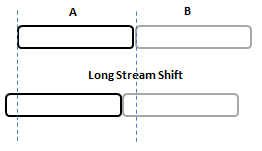
\includegraphics[scale=0.8]{draw/long_shift.png}
\caption{Long stream shifting}
\label{fig:long_shift}
\end{figure}

\begin{figure}[htbp!]
\centering
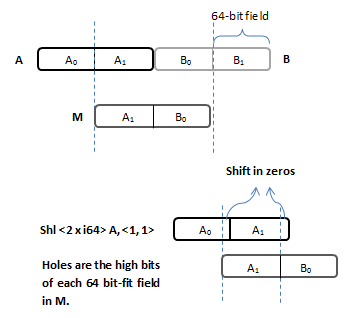
\includegraphics[scale=0.9]{draw/long_shift_good.png}
\caption{A better algorithm for long stream shift.}
\label{fig:long_shift_good}
\end{figure}

We first show a peephole optimization that greatly improves the performance of long stream shifting. Long stream shifting shifts left one whole SIMD register with potential shift-in bits from the other SIMD register. Refer to Figure~\ref{fig:long_shift}, we want to shift left {\tt A} by $n$ bits and shift-in the highest $n$ bits from B. For simplicity, we assume $n = 1$ and the SIMD register is 128-bits wide. The most straight-forward implementation is listed below:
  \[ \text{\tt A1 = shl i128 A, 1} \]
  \[ \text{\tt B1 = lshr i128 B, 127} \]
  \[ \text{\tt R = or i128 A1, B1} \]
This algorithm is called double shift. It describes clearly what we want to implement so it is the preferred IR code in the library. Since shift on $i128$ is not natively supported, double shifts of $v2i64$ and one shufflevector are needed to implement the $i128$ shift. Thus, we need 4 $v2i64$ shifts, 2 shufflevectors and 3 logic or operations.

\begin{figure}[htbp!]
\centering
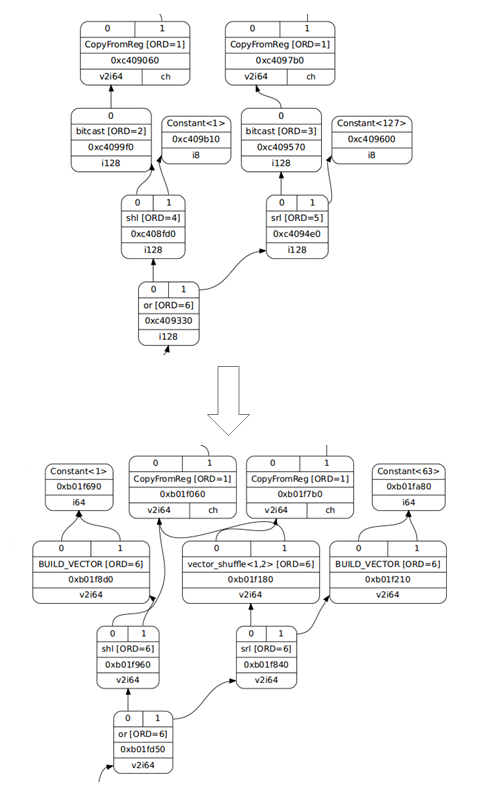
\includegraphics[scale=0.8]{draw/long_shift_nodes.png}
\caption[The DAG combiner for long stream shift.]{The DAG combiner for long stream shift. When the above pattern is recognized, it gets replaced with the better implementation below.}
\label{fig:long_shift_nodes}
\end{figure}

A better algorithm that uses 2 $v2i64$ shifts, 1 shufflevector and 1 logic or is implemented. Refer to Figure~\ref{fig:long_shift_good}, the algorithm is listed below:
  \[ \text{\tt M = shufflevector <2 x i64> A, B, <2 x i32> <i32 1, i32 2>} \]
  \[ \text{\tt D = shl <2 x i64> A, <2 x i64> <i32 1, i32 1>} \]
  \[ \text{\tt E = lshr <2 x i64> M, <2 x i64> <i32 63, i32 63>} \]
  \[ \text{\tt R = or <2 x i64> D, E} \]

{\tt M} is the key to this algorithm. When we shift left {\tt A} as $v2i64$, we create holes (1-bit shift-in zeros) in the lower end of each field. The correct fill-in data for these holes are just the highest bit in each field of {\tt M}. So we shift right {\tt M} as $v2i64$ to align the bits into correct positions and use logic or operation to fill the holes. This algorithm can be generalized to long stream shift of an arbitrary amount.

Once the back end recognizes the double-shift code, it re-implements with the latter algorithm. The DAG combining process is described in Figure~\ref{fig:long_shift_nodes}.

The next example is shufflevector for {\tt hsimd<16>::packh}. With the similar code described in Chapter~\ref{three}, LLVM 3.4 does not generate the best assembly code. It generates a sequence of $pextrw$ and $pinsrw$. Even the newst LLVM truck generates 27 lines of assembly. We create the following DAG Combiner and get the 5 lines of equivalent assembly code in Program~\ref{prog:packh_16_asm}.
\begin{itemize}
    \item \textbf{Pattern}: shufflevector on $v16i8$ with mask = 1, 3, 5, \ldots, 31.
    \item \textbf{Combine Result}: one PACKUS node, which unsigned saturates two $v8i16$ into $v8i8$ vectors and concatenates them into one $v16i8$.
\end{itemize}

\begin{program}[htbp!]
\begin{verbatim}
    psrlw   $8, %xmm0
    psrlw   $8, %xmm1
    packuswb    %xmm0, %xmm1
    movdqa  %xmm1, %xmm0
    retq
\end{verbatim}
\caption{The optimized assembly code for {\tt hsimd<16>::packh}}
\label{prog:packh_16_asm}
\end{program}

\FloatBarrier
The efficient implementation of {\tt packh} on vectors of small elements are possible with the PEXT instruction introduced by the Intel Haswell BMI2. PEXT is a useful instruction for bit manipulation on $i32$ and $i64$. Given the $i8$ variable A = $(\text{abcdefgh})_2$, Mask = $(10101010)_2$, PEXT(A, Mask) returns R = $(\text{aceg})_2$. PEXT extracts bits from A at the corresponding bit locations specified by the mask. With this in mind, we can implement \verb|hsimd<2>::packh| as Program~\ref{program:packh_2} (in pseudo IR for readability).

\begin{program}[htbp!]
\begin{verbatim}
    define <2 x i64> @packh_2(<2 x i64> A, <2 x i64> B) {
    entry:
      ; extract lower 64 bits (A0) and higher 64 bits (A1)
      A0 = extractelement <2 x i64> A, i32 0
      A1 = extractelement <2 x i64> A, i32 1

      Mask = 0xAAAAAAAAAAAAAAAA ; 1010...1010 in binary
      P0 = PEXT(A0, Mask) | (PEXT(A1, Mask) << 32)

      ; same for B
      B0 = extractelement <2 x i64> B, i32 0
      B1 = extractelement <2 x i64> B, i32 1
      P1 = PEXT(B0, Mask) | (PEXT(B1, Mask) << 32)

      ret <2 x i64> <i64 P0, i64 P1>
    }
\end{verbatim}
\caption{Implementation of {\tt hsimd<2>::packh} with PEXT.}
\label{program:packh_2}
\end{program}

According to Program~\ref{program:packh_2}, we create the following DAG Combiner:
\begin{itemize}
    \item \textbf{Pattern}: shufflevector on $v128i1$, $v64i2$ or $v32i4$ with mask = 0, 2, 4, \ldots, $NumElt \times 2-2$ or mask = 1, 3, 5, \ldots, $NumElt \times 2 -1$. $NumElt$ is the number of elements for each type e.g.\ $NumElt=32$ for $v32i4$.
    \item \textbf{Combine Result}: four PEXT nodes combined with OR and SHL.
\end{itemize}

To summarize, this kind of DAG Combiner provides a shortcut for the programmer to do peephole optimization. It can co-exist with a full custom lowering, like the relationship between immediate shifting and arbitrary shifting. Immediate shifting shifts all the vector elements by the same amount, allowing efficient realization for $v32i4$ with $v4i32$ shifts, while we apply the In-place Promotion strategy for $v32i4$ arbitrary shifting in the Parabix custom lowering.

DAG Combiner can optimize operations with illegal types in the phase DAG Combine 1. It is not possible in the custom lowering. But we cannot simply put all the Parabix Custom Lowering logic inside the DAG Combiner. First, it is against LLVM design; DAG Combiner is designed for cleaning up, either the initial code or the messy code generated by the legalization passes \cite{llvm_code_gen}. Second, it cannot utilize the legalization iteration; in custom lowering, general strategies may introduce new illegal operations which are hard to avoid since ``illegal" is a target-specific concept. The DAG Combiner, on the other hand, 1) should not generate illegal operations in the phases after the operation legalization phase, 2) although it can also work in iteration, most of the lowering logic for common operations are not programmed in this module, we would end up with illegal non-Parabix operations.

\section{Templated Implementation}
During our implementation, we encountered a lot of duplicated code, especially in the test cases; Such duplication is against software design principles and is hard to maintain, sometimes even hard to write; a thorough test file for $i2^k$ vector contains more than two thousand lines of code, most of which are in the same pattern. To keep DRY and save programmer time, we introduced the Jinja template engine \cite{jinja_engine}. According to \cite{python_templating}, Jinja belongs to the Engines Mixing Logic into Templates, it allows embedding logic or control-flow into template files. We use Jinja because:

\begin{itemize}
    \item We can write all pieces of the content in one file, so it is easier to understand. Where in the Engines using Value Substitution, the driver code usually contains many tiny pieces of content. The reader must read the driver code as well as the template file to understand the output. One template example can be found in Program~\ref{program:jinja}.
    \item Like the standard Model-View-Controller structure in the web design, our driver code needs only provide abstract data (like operation names in IR and the corresponding C++ library calls). How to present these data is not its responsibility. In the other words, we can have significant changes in the template without changing the driver.
    \item Jinja uses python and python is easy and quick to use.
\end{itemize}

\subsection{Code Generation For $i2$ Vector}
In Chapter~\ref{four}, we legalized $i2$ vector operations with boolean functions. In our implementation, with the Quine-McCluskey solver, we got 11 sets of formulas which reside in one compact data script. We wrote template files to generate 11 C++ functions for them. This approach has the following benefits:
\begin{itemize}
    \item It collects all the critical formula together so that possible future updates are easy to deploy.
    \item Implementation details only reside in the template file, so we are able to change the code structure easily. For now we create one function for each formula, but it is possible that we could create one big switch statement and generate one case for each formula instead. This can be done with only a few lines of change in the template.
\end{itemize}

Example formula of $v64i2$ addition as well as the function template is listed in the Program~\ref{prog:i2_codegen} and Program~\ref{prog:i2_func_template}.

\begin{program}[htbp!]
\begin{verbatim}
    "add_2": r'''
        tmp = simd_xor(arg1, arg2)
        return simd_ifh1(simd_himask(fw),
                         simd_xor(tmp, simd_slli(1, simd_and(arg1, arg2))), tmp)
    '''
\end{verbatim}
\caption[Minimum boolean function for $v64i2$ addition]{Minimum boolean function for $v64i2$ addition.}
\label{prog:i2_codegen}
\end{program}

\begin{program}[htbp!]
\begin{verbatim}
    
    /* Generated function */
    static SDValue GENLower{{ name.op }}(SDValue Op, SelectionDAG &DAG) {
      MVT VT = Op.getSimpleValueType();
      MVT FullVT = getFullRegisterType(VT);
      SDNodeTreeBuilder b(Op, &DAG);

      if (VT == MVT::v64i2) {
        SDValue A1 = b.BITCAST(Op.getOperand(0), FullVT);
        SDValue A2 = b.BITCAST(Op.getOperand(1), FullVT);

    
        {{ line | trim }};
    
      }

      llvm_unreachable("GENLower of {{ name.op }} is misused.");
      return SDValue();
    }

    
\end{verbatim}
\caption[Custom lowering function template for $v64i2$]{Custom lowering function template for $v64i2$. This template file generates one function for each operation.}
\label{prog:i2_func_template}
\end{program}

\subsection{Test Code And IR Library Generation}
We test correctness of our modified LLVM back end by comparing results with the IDISA library. For example we extend LLVM to support $i1$ vectors, but does the extention work? We answer this question by first constructing a IR library of all the functions on $i1$ such as the {\tt add\_1} listed in the top left corner in Figure~\ref{figure:test}. We then write a driver to generate random test data, put them through the IR functions as well as the corresponding IDISA functions, and check if the results are the same.

There is one problem in this approach. The driver and IDISA are both written in C++ but the IR library is in low-level representation. How to mix them together? We solve the problem by compiling the IR code into object files. A seperate header file of IR-function signatures is maintained so that the driver code can call IR functions as external functions. The overview of the test system can be found in Figure~\ref{figure:test}. We use templates for both the IR library and the driver, some sample templates can be found in Program~\ref{program:jinja}.


\begin{figure}[hbpt!]
\centering
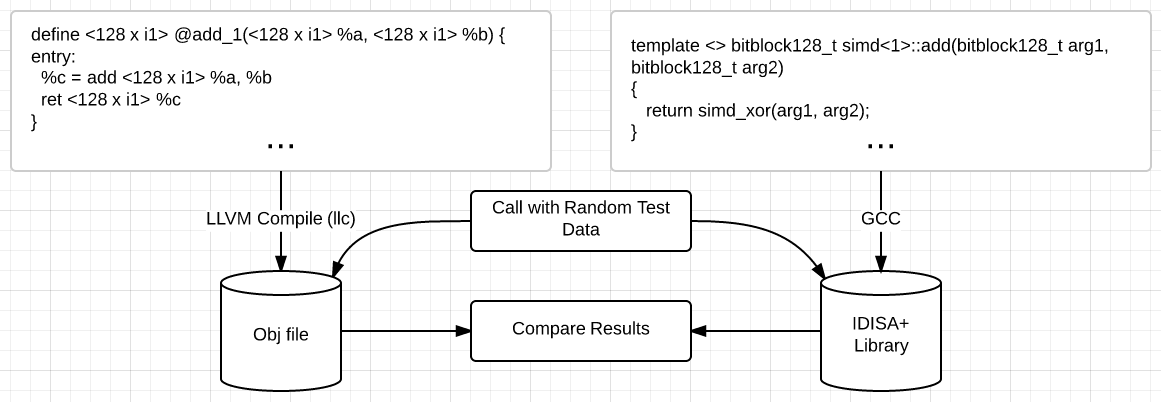
\includegraphics[width=140mm]{draw/test.png}
\caption[Test system overview.]{Test system overview. The pure IR library is first compiled into the native object file and then linked with the driver. The driver call functions from the both side to check correctness.}
\label{figure:test}
\end{figure}

\begin{program}
\begin{verbatim}

define <32 x i4> @{{name.c}}(<32 x i4> %a,
                             <32 x i4> %b)
{
entry:
  %c = {{ name.op }} <32 x i4> %a, %b
  
  %d = sext <32 x i1> %c to <32 x i4>
  ret <32 x i4> %d
  
  ret <32 x i4> %c
  
}

\end{verbatim}
\rule{\textwidth}{1pt}

\begin{multicols}{2}
\begin{verbatim}
define <32 x i4> @add_4(<32 x i4> %a,
                        <32 x i4> %b)
{
entry:
  %c = add <32 x i4> %a, %b
  ret <32 x i4> %c
}
\end{verbatim}
\columnbreak
\begin{verbatim}
define <32 x i4> @eq_4(<32 x i4> %a,
                       <32 x i4> %b)
{
entry:
  %c = icmp eq <32 x i4> %a, %b
  %d = sext <32 x i1> %c to <32 x i4>
  ret <32 x i4> %d
}
\end{verbatim}
\end{multicols}
\caption[Templates for the IR Libray]{Templates for the IR Library. On the top is the template, and two different output are listed below. We use embedded for loop and if statements.}
\label{program:jinja}
\end{program}

%%%%%%%%%%%%%%%%%%%%%%%%%%%%%%%%%%%%%%%%%%%%%%%%%
%
%     Chapter 6
%
%%%%%%%%%%%%%%%%%%%%%%%%%%%%%%%%%%%%%%%%%%%%%%%%

\chapter{Performance Evaluation}
\label{six}

In this chapter, we focus on the performance evaluation to assess whether our LLVM back end matches the performance of the hand-written library and whether back end optimizations provide performance advantages. We first validate our vector of $i2^k$ approaches, and then present the performance of some critical Parabix operations via an application-level profile.

\section{Vector of $i2^k$ Performance}
In Chapter~\ref{four}, we presented different approaches to lower $i1$, $i2$, $i4$ and some $i8$ operations within one SIMD register. In this section, we validate our approaches by showing the improved run-time performance.

\subsection{Methodology}

Testing small pieces of critical code can be tricky, since the testing overhead can easily overwhelm the critical code and make the result meaningless. Agner Fog provides a test program which uses the Time Stamp Counter for clock cycles and Performance Monitor Counters for instruction count and other related events \cite{agner_testp}. We pick the reciprocal throughput as our measurement. It is measured with a sequence of same instructions where subsequent instructions are independent of the previous ones. In Fog's instruction table, he noted that a typical length of the sequence is 100 instructions of the same type and this sequence should be repeated in a loop if a larger number of instructions is desired.

We did one simple experiment with SIMD XOR ($xorps$) to validate this program. In Figure~\ref{figure:testp_xor}, we show the measured performance of executing different number of XOR instructions; they are organized into one for loop. We have checked the assembly code to make sure the XOR operations are not optimized away.

\begin{figure}[ht!]
\centering
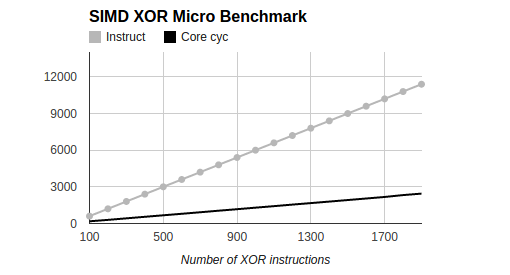
\includegraphics[width=140mm]{draw/testp_xor.png}
\caption[Test Performance with XOR]{Test performance with XOR\@. The dotted line is instruction count and the other line is core CPU cycles.}
\label{figure:testp_xor}
\end{figure}

From the figure, we can see the instruction count and CPU cycles grows linearly with the number of XOR instructions. So we can conclude that Fog's test program can be used to compare two pieces of critical code: the one with more measured CPU cycles is more complex and has more instructions. Note that from the figure, it seems the throughput of $xorps$ is 4, which is different from Intel's document (3.0 in document). We found this may be related to the compiler optimization on the loop; when we flattened the loop we got the throughput around 2.7. In order to eliminate this undesired effect, we flatten all the test code in the following sections.

In the following sections, we write micro benchmarks with Agner Fog's test program and compare reciprocal throughput between different implementation. Our test machine is X86 64-bit Ubuntu with Intel Haswell, and the detailed configuration can be found in Table~\ref{table:hardware_config}. In order to inline pure IR functions (instead of a function call into one object file), we compile all the test code into LLVM bit code (binary form of LLVM IR) and then link / optimize them together. The default compile flag is to use Intel SSE2 instruction set on the 64-bit OS.

\begin{table}[h]
\centering
\begin{tabular}{|c|c|}
\hline
CPU Name       & Intel(R) Core(TM) i5-4570 CPU \\ \hline
CPU MHz        & 3200                          \\ \hline
FPU            & Yes                           \\ \hline
CPU(s) enabled & 4 cores                       \\ \hline
L1 Cache       & 32 KB D + 32KB I              \\ \hline
L2 Cache       & 256 KB                        \\ \hline
L3 Cache       & 6 MB                          \\ \hline
Memory         & 8GB                           \\ \hline
\end{tabular}
\caption{Hardware Configuration}
\label{table:hardware_config}
\end{table}

\begin{table}[h]
\centering
\begin{tabular}{|c|c|}
\hline
Operating System & Ubuntu (Linux X86-64)         \\ \hline
Compiler         & Clang 3.5-1ubuntu1, GCC 4.8.2 \\ \hline
LLVM             & LLVM 3.5                      \\ \hline
File System      & Ext4                          \\ \hline
\end{tabular}
\caption{Software Configuration}
\label{table:software_config}
\end{table}

\subsection{Performance Against IDISA}
We compare our lowering on pure IR functions with the IDISA Library \cite{hua_idisa} which is written in C++. To test each operation, we generate a sequence of 500 such operations where none them has to wait for the previous one. 100 operations which are suggested by Agner seems too short for a stable result. This test sequence is generated by a template file.

For completeness, we choose all the operations listed in Table~\ref{table:semantics} except: NE (not equal), because IDISA does not support this operation; shifts (SRL, SRA, SHL) because IDISA only supports immediate shifts while the IR library supports arbitrary shifts; the comparison is not fair; bitwise-logic (AND, OR, XOR), because the underline implementation are exactly the same and as simple as one line of machine code; we remove them to simplify the test code. Finally, we get eight operations for the micro-benchmark: ADD, SUB, MULT, EQ, LT, GT, ULT and UGT.

The performance comparison is listed in Figure~\ref{figure:throughput_vector} and Figure~\ref{figure:cpu_cycles_vector}. We can see for $i1$ and $i4$ vectors, the IR library has the similar performance with IDISA but it performs better with $i2$ vectors, especially on integer comparison.

The underlying logic for both libraries is the same, but it is implemented in different levels. For the IDISA library, {\tt simd<2>::ugt} is inline-extended immediately by the compiler front end and its semantics of integer comparison lost ever after, while in the IR library, for the whole life cycle before the instruction selection, {\tt ugt\_2} keeps its semantics. The extension of {\tt ugt\_2} is delayed until the instruction selection phase, right before machine code generation. And the delayed extension may help the compiler optimize as we discussed in Chapter~\ref{three}. We checked that the IDISA function {\tt simd<2>::ugt} and IR function {\tt ugt\_2} (whose underlying code is just \verb|icmp ugt <64 x i2> %a, %b|) generated different assembly code.

\begin{figure}[htbp!]
\centering
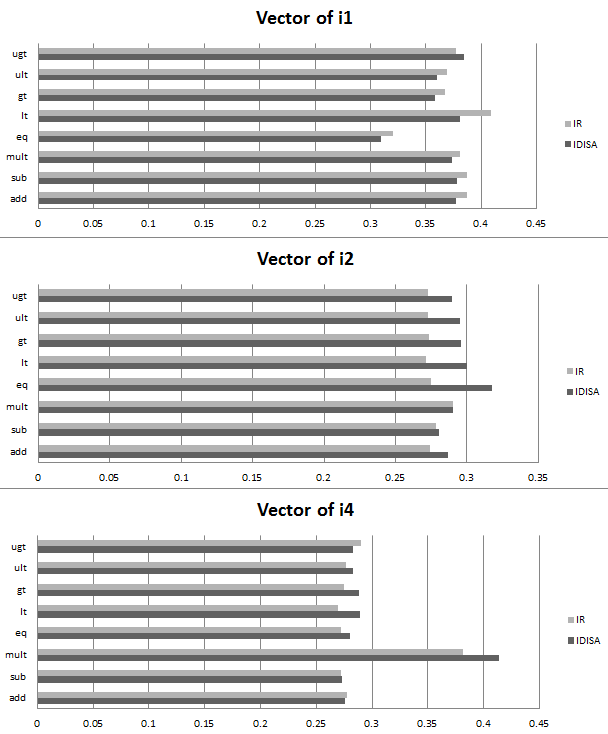
\includegraphics[width=140mm]{draw/reciprocal_throughput_vector.png}
\caption[Reciprocal instruction throughput against IDISA library]{Reciprocal instruction throughput against IDISA library. IR and IDISA share almost identical throughput.}
\label{figure:throughput_vector}
\end{figure}

\begin{figure}[htbp!]
\centering
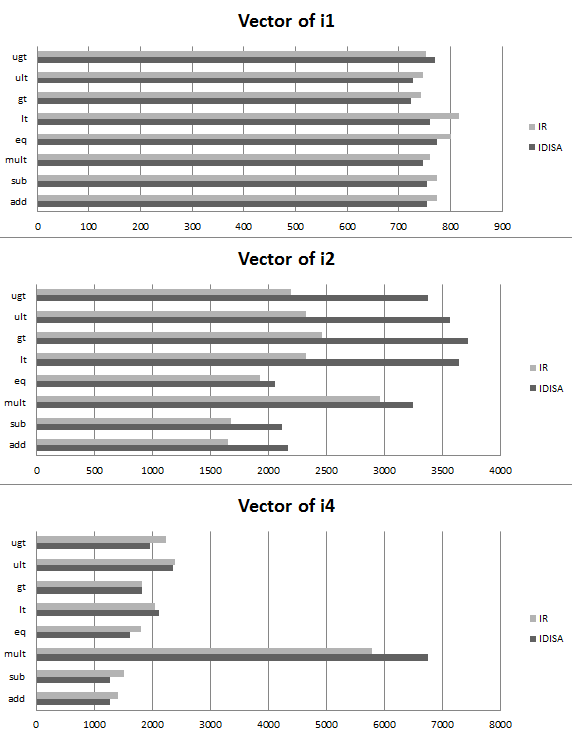
\includegraphics[width=140mm]{draw/cpu_cycles_vector.png}
\caption[Total CPU cycles against IDISA library]{Total CPU cycles against IDISA library; for $i1$ and $i4$ vectors, IR library has the similar performance with IDISA but it performs better with $i2$ vectors, especially on integer comparison.}
\label{figure:cpu_cycles_vector}
\end{figure}

However, the delay in expansion is not always good. Take multiplication on the $i2$ vector for an example, we can see our IR library has slightly bettered total CPU cycles, but if we write our instructions sequence with a loop, IDISA library wins (Figure~\ref{figure:loop_vector_i2}). Loop optimization is responsible for this difference; we did observe lines of assembly code hoisted outside the loop. Because all the operations tested here take two operands and the same constant value is used for all the second operand for simplicity, there is duplicated logic in each loop iteration that can be hoisted and shared. Hoisting was not done with the IR library. So early expansion in IDISA provides some optimization opportunity to the compiler.

From the reciprocal throughput comparison (Figure~\ref{figure:throughput_vector}), the IR library loses on $i1$ vectors but wins most of the cases in $i2$ and $i4$; it may relate to a better instruction selection. IDISA library is generated from a strategy pool based on the number of machine instructions which are treated equally with cost 1. But machine instructions actually have different throughput in the real hardware, and the LLVM back end has more knowledge of that, thus selecting better instructions.

\begin{figure}[htbp!]
\centering
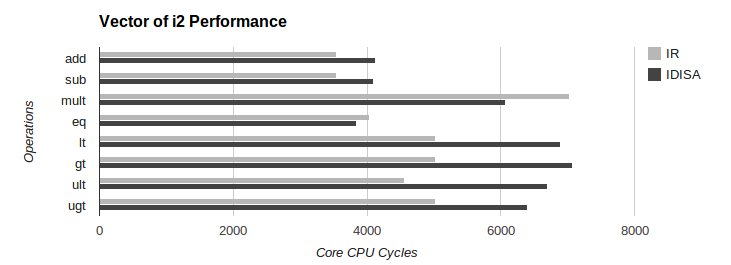
\includegraphics[width=140mm]{draw/loop_vector_i2.png}
\caption[Vector of $i2$ tested in a loop]{The same benchmark for $i2$ vectors with the instruction in a loop. Code in Figure~\ref{figure:cpu_cycles_vector} can be seen as the flattened version of this figure. We find IDISA here wins in the multiplication on $i2$, while IR wins it in Figure~\ref{figure:cpu_cycles_vector}. Loop optimization should be responsible for it.}
\label{figure:loop_vector_i2}
\end{figure}

\subsection{Performance Against LLVM}
We compare our lowering with native LLVM\@. LLVM could not handle $i2$, $i4$ vectors but could handle $i1$ vectors slowly. Detailed performance data can be found in Table~\ref{table:vector_perf_LLVM}. We can see that our approach fills the gap of the LLVM type system.

\begin{table}[h]
\centering
\begin{tabular}{|c|c|c|c|c|}
\hline
     & $i1$ & $i2$ & $i4$ & $i8$ \\ \hline
add  & 302  & X    & X    & 1\\ \hline
sub  & 310  & X    & X    & 1\\ \hline
mult & X    & X    & X    & 10\\ \hline
eq   & 273  & X    & X    & 1\\ \hline
lt   & X    & X    & X    & 1\\ \hline
gt   & X    & X    & X    & 1\\ \hline
ult  & 349  & X    & X    & 1\\ \hline
ugt  & 290  & X    & X    & 1\\ \hline
\end{tabular}
\caption[Performance against LLVM native support for $i2^k$ vectors]{Performance against LLVM native support of $i2^k$ vectors. `X' means compile error or compile too slowly (longer than 30s), the remaining number means the ratio of CPU cycles speed up: add takes 302 times of cycles that our lowering needs. For $i8$, we apply the inductive doubling strategy on the multiplication, which explains the 10 times speed up. }
\label{table:vector_perf_LLVM}
\end{table}

\section{Parabix Critical Operations}
In this section, we evaluate our work by replacing Parabix critical operations with the IR library. We first choose transposition and inverse transposition as two representative operations and then measure performance in two Parabix applications: XML validator and UTF-8 to UTF-16 transcoder. Note that we did not rewrite the whole application with an IR library, part of the application is still IDISA but some critical operations are replaced. The default compile flag is to use the Intel SSE2 instruction set on a 64-bit OS.

To compare performance, we use the same data files used in \cite{rob_xml}. The description of these files can be found in Table~\ref{table:xmlwf_data}.

\begin{table}[h]
\centering
\begin{tabular}{|c|c|c|c|c|c|}
\hline
File Name           & dew.xml & jaw.xml & roads-2.gml & po.xml  & soap.xml \\ \hline
File Type           & document   & document   & data      & data    & data     \\ \hline
File Size (MB)      & 66      & 7       & 11    & 76   & 3     \\ \hline
Markup Item Count   & 406k     & 74k      & 280k    & 4634k & 18k    \\ \hline
Attribute Count     & 18k      & 3k       & 160k    & 463k  & 30k    \\ \hline
Avg. Attribute Size & 8          & 8          & 6         & 5       & 9        \\ \hline
Markup Density      & 0.07       & 0.13       & 0.57      & 0.76    & 0.87     \\ \hline
\end{tabular}
\caption{XML Document Characteristics. Taken from \cite{rob_xml}.}
\label{table:xmlwf_data}
\end{table}

\begin{table}[h]
\centering
\begin{tabular}{|c|c|c|c|c|c|}
\hline
        & dew.xml  &  jaw.xml  &  roads-2.gml  &  po.xml  & soap.xml¬ \\\hline
xmlwf0   &  3.93   &    4.36   &   4.55   &   4.89   &   5.18 \\ \hline
xmlwf0 on Haswell   &  3.92   &   4.36   &   4.55   &   4.87   &   5.17 \\ \hline

xmlwf1   &  3.92   &   4.37   &   4.56   &   4.86   &   5.18 \\ \hline
xmlwf1 on Haswell &   3.56   &   3.97   &   4.16   &   4.45   &   4.78 \\ \hline
\end{tabular}
\caption[Performance comparison of XML Validator (xmlwf)]{Performance comparison of XML validator (xmlwf), in a thousand CPU cycles per thousand byte. In the table, xmlwf0 is implemented with full IDISA library and xmlwf1 is a copy of xmlwf0 with the transposition replaced.}
\label{table:xmlwf_perf}
\end{table}

\begin{table}[h]
\centering
\begin{tabular}{|c|c|c|c|c|c|}
\hline
 & dew.xml & jaw.xml & roads-2.gml & po.xml & soap.xml \\ \hline
 U8u16\_0         & 281.46  & 37.11   & 40.06       & 244.94 & 10.20    \\ \hline
 U8u16\_0 Haswell & 272.68  & 34.21   & 39.84       & 242.56 & 10.11    \\ \hline
 U8u16\_1         & 284.17  & 36.71   & 41.65       & 255.57 & 10.60     \\ \hline
 U8u16\_1 Haswell & 267.14  & 34.64   & 38.53       & 237.66 & 9.98     \\ \hline
 \end{tabular}
 \caption[Performance comparison of UTF-8 UTF-16 Transcoder]{Performance comparison of UTF-8 UTF-16 transcoder, in a million CPU cycles. U8u16\_0 is written in IDISA, U8u16\_1 has the transposition and inverse transposition part replaced.}
 \label{table:u8u16_perf}
 \end{table}

Table~\ref{table:xmlwf_perf} shows the performance of the XML Validator. The only difference of xmlwf0 and xmlwf1 is their transposition code. The one in xmlwf1 is written in pure IR with the byte-pack algorithm (the source code can be found in Appendix~\ref{appone:transposition}). We can see xmlwf0 and xmlwf1 share almost identical performance but it is not for free. LLVM 3.4 cannot handle packing on 16-bit field width very well so we custom lower the shufflevector and generate PACKUS instructions for X86.

Another interesting observation is, when we re-compiled the same code on the Intel Haswell platform, we got almost no improvement for xmlwf0, since the IDISA library linked in is written with direct SSE2 intrinsic so only SSE2 instructions can be generated. But we got a slightly better performance for xmlwf1, because the IR library is target-independent. LLVM back end knows AVX2 is available so it generates VEX prefixed operations with three-operand form.

Similar performance data on the UTF-8 to UTF-16 transcoder is listed in Table~\ref{table:u8u16_perf}. U8u16\_0 is written in IDISA and U8u16\_1 has both the transposition and inverse transposition part replaced. Since our modified LLVM could not generate machine code as good as IDISA, there are performance drops from U8u16\_0 to U8u16\_1. We also tried to compile them on the full Haswell, which gave us similar performance benefit from using AVX2 VEX operations. The feature of being target-independent helps Parabix to enjoy the improvement of hardware without changing its source code.

\subsection{Ideal 3-Stage Transposition on the Intel Haswell}
Intel Haswell architecture introduces the PEXT operation which can be used for the ideal 3-stage transposition (source code in Appendix~\ref{appone:transposition_ideal}). We evaluated its performance in Table~\ref{table:PEXT_transposition}. The performance dropped with PEXT, but the major reason is that PEXT can only work on $i32$ or $i64$ integers for the current architecture. As the hardware evolves, we may have PEXT on SIMD registers directly. At that time, we can expect a better performance in xmlwf2, may be better than both xmlwf0 and xmlwf1 since 3-stage transposition is proved to be optimal under the IDISA model \cite{inductive_doubling_principle}. Our approach provides a new chance to exploit future hardware improvements.

\begin{table}[h]
\centering
\begin{tabular}{|c|c|c|c|c|c|}
\hline
        & dew.xml  &  jaw.xml  &  roads-2.gml  &  po.xml  & soap.xml¬ \\\hline
xmlwf0 on Haswell   &  3.92   &   4.36   &   4.55   &   4.87   &   5.17 \\ \hline
xmlwf1 on Haswell &   3.56   &   3.98   &   4.16   &   4.45   &   4.78 \\ \hline
xmlwf2 on Haswell & 4.11   &    4.49   &    4.69   &    4.97   &   5.30 \\ \hline
\end{tabular}
\caption[Ideal 3-Stage Transposition with PEXT]{Performance of the ideal 3-stage transposition in a thousand CPU cycles per thousand byte. Xmlwf2 uses the ideal 3-stage transposition algorithm. Xmlwf1 uses byte-pack algorithm in IR, xmlwf0 uses the same algorithm in IDISA.}
\label{table:PEXT_transposition}
\end{table}

\subsection{Long Stream Addition And Shift}
We replaced the internal logic of big integer addition in Chapter~\ref{four} and introduced a new intrinsic: {\tt uadd.with.overflow.carryin}. We evaluate them in this section by first comparing the long-stream addition algorithm with LLVM's original implementation and then some application level profiles for the new intrinsic.

We wrote micro benchmarks with Fog's test program. We put 200 independent additions on $i128$ and $i256$. We choose 200 because 200 is a small number that can give us stable performance results. It was tricky to make the test program right; we generated random data for the operands and carefully inserted the carry-out bit back to the return value so that LLVM knows to use the long-stream-addition logic. In order to be consistent throughout the comparison, we used the same compiler flag for all the runs ({\tt -mavx2} for gcc and {\tt -mattr=+avx2,+bmi2} for LLVM tool chain). The result is listed in Table~\ref{table:lsadd_micro}.

\begin{table}[h]
\centering
\begin{tabular}{|c|c|c|}
\hline
                             & Core CPU Cycles & Instructions \\ \hline
Long stream addition on $i128$ & 2416            & 6552         \\ \hline
LLVM on $i128$                 & 1455            & 4199         \\ \hline
Long stream addition on $i256$ & 2656            & 6959        \\ \hline
LLVM on $i256$                 & 4234            & 9798         \\ \hline
\end{tabular}
\caption{Micro benchmarks for long stream addition against LLVM's original implementation.}
\label{table:lsadd_micro}
\end{table}

Long stream addition does not perform well on $i128$. Since there are only two sequential additions involved (1 $addq$ and 1 $adcq$), parallel computing does not save much but introduces new complexity. However, on $i256$ long stream addition has much better performance than the sequential one which generates 1 $addq$ and 3 $adcq$. As the width of the operand doubles, the CPU cycles from LLVM increases to the rate of 2.91, while in the long stream addition, the rate is only 1.10. This is because the time complexity of our algorithm is independent of the operand size while the sequential one has the time complexity linear to the operand size. Our algorithm scales better when the width of SIMD registers grows. We can confidently predict that on the Intel AVX512, long stream addition on $i512$ would out-perform the sequential one significantly.

An important Parabix application is regular expression matching. A grep-like tool was written recently with bitwise data parallelism called `icgrep' \cite{dale_icgrep}. Icgrep uses LLVM just-in-time compiling facility to generate IR code on the fly according to the input regular expression. We use icgrep to evaluate our new intrinsic for long stream addition. Its signature is in Program~\ref{prog:uadd_carryin} and it is used for the "add with carry" logic in icgrep.

\begin{program}[htbp!]
\begin{verbatim}
  {i128, i1} @llvm.uadd.with.overflow.carryin.i128(i128 %a, i128 %b, i1 %carryin)
  ; return a pair of sum and carry-out bit
\end{verbatim}
\caption[Signature of {\tt uadd.with.overflow.carryin}]{Signature of {\tt uadd.with.overflow.carryin}.}
\label{prog:uadd_carryin}
\end{program}

To compare with the unmodified LLVM, we need to emulate this new intrinsic. LLVM supports {\tt uadd.with.overflow} which does not take the carry-in bit into account. The pseudo code for "add with carry" is listed in Program~\ref{prog:uadd}. Then we can compare our back end with the unmodified LLVM\@. The same regular expressions and data files are used in \cite{rob_regex}. Since we only care about the improvement between back ends, the details of the regular expressions are not important. We show the relative instruction counts in Figure~\ref{fig:inst_count_long_add}. The experiment was done with 128-bit SIMD registers and most of the improvement comes from the fact that our back end only requires one addition.

\begin{program}[htbp!]
\begin{verbatim}
  declare {i128, i1} @llvm.uadd.with.overflow.i128(i128 %a, i128 %b)
  ;return a pair of sum and carry-out bit

  {i128, i1} @add_with_carry(i128 %a, i128 %b, i1 %carryin) {
  entry:
    cin = zext %carryin to i128

    {s1, c1} = @llvm.uadd.with.overflow.i128(%a, %b)
    {sum, c2} = @llvm.uadd.with.overflow.i128(s1, cin)

    cout = or i1 c1, c2
    ret {sum, cout}
  }
\end{verbatim}
\caption[Pseudo code for "add with carry" logic in with unmodified LLVM]{Pseudo code for "add with carry" logic in with unmodified LLVM\@.}
\label{prog:uadd}
\end{program}

\begin{figure}[htbp!]
\centering
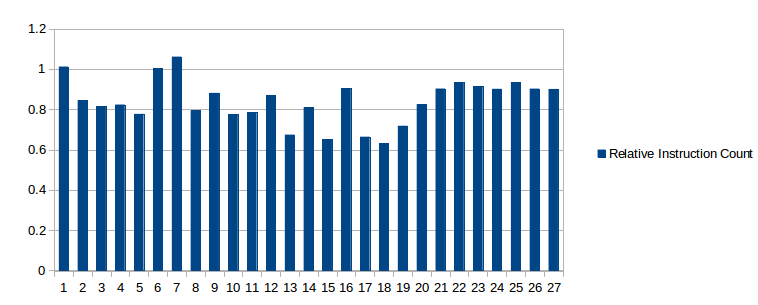
\includegraphics[width=140mm]{draw/inst_count_long_add.png}
\caption[Improvement with long stream addition and the new intrinsic in instruction count]{Improved instruction count with long stream addition. The number in the figure is the ratio of the instruction count in our back end to the count in unmodified LLVM. 27 pairs of regular expressions and data files are evaluated.}
\label{fig:inst_count_long_add}
\end{figure}

We then compare the long stream shifting algorithms. We discussed two algorithms in Section~\ref{sec:long_shift}; we implemented a DAG combiner in our back end. IR code of double shift can be compiled on the unmodified LLVM, so it is convenient that no new source code needs to be written. We used exactly the same code on both of the back ends. To avoid a difference in "add with carry", we used a logic that generates the same machine code on both back ends. The comparison of long stream shifting with 128-bit SIMD registers is listed in Figure~\ref{fig:inst_count_long_shift}. We can see a reduction of 10 to 20 percent in instructions.

\begin{figure}[htbp!]
\centering
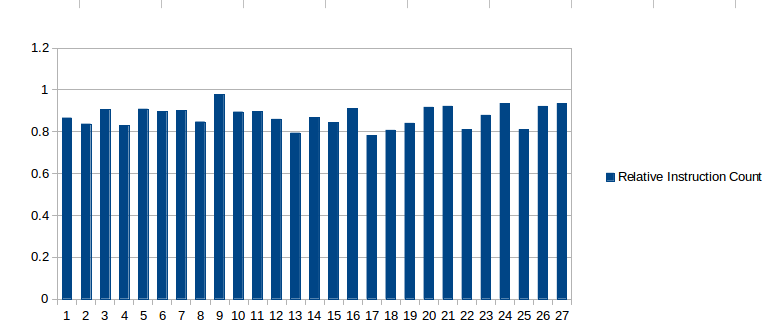
\includegraphics[width=140mm]{draw/inst_count_long_shift.png}
\caption[Improvement with long stream shifting in instruction count]{Improvement with long stream shifting in instruction count. The number in the figure is the ratio of the instruction count in our back end to the count in unmodified LLVM.}
\label{fig:inst_count_long_shift}
\end{figure}

Finally, we study the behaviour of long stream addition and shifting with 256-bit SIMD registers. We turned on both of the optimizations for icgrep. The relative instruction count is listed in Figure~\ref{fig:inst_count_all_256}. From the micro-benchmark we already know that long stream addition works better than the sequential addition on this wider SIMD register. Together with long stream shifting, we achieved a significant 30 to 40 percent instruction reduction against the unmodified LLVM.

\begin{figure}[htbp!]
\centering
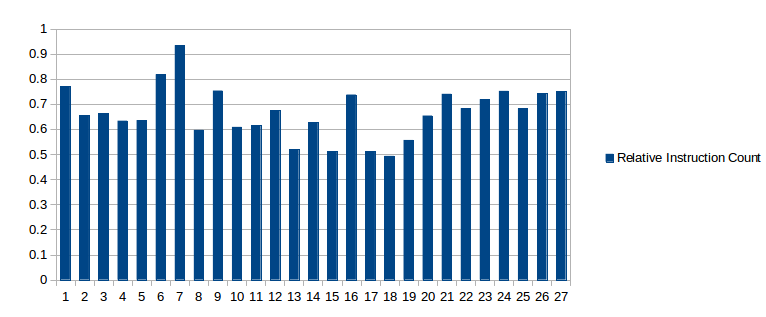
\includegraphics[width=140mm]{draw/inst_count_all_256.png}
\caption[Improvement of icgrep on machines with 256-bit SIMD registers]{Improvement of icgrep on machines with 256-bit SIMD registers. Both long stream shifting and addition are used. The instruction count is compared with the unmodified LLVM with 256-bit SIMD registers.}
\label{fig:inst_count_all_256}
\end{figure}

%%%%%%%%%%%%%%%%%%%%%%%%%%%%%%%%%%%%%%%%%%%%%%%%%
%
%     Chapter 7
%
%%%%%%%%%%%%%%%%%%%%%%%%%%%%%%%%%%%%%%%%%%%%%%%%

\chapter{Conclusion}
\label{seven}

In this thesis, we demonstrated that it is possible to extend LLVM type system to support Parabix technology. We have shown systematic support of the vector of $i2^k$ and support of critical Parabix operations in the target-independent IR library. We have also shown in one specific target: Intel X86, we can generate efficient native code. We added a new LLVM intrinsic that enables chained additions on long bit streams, which can be used for a broad category of applications.


%%%%%%  bibliography
%% Copyright 1998 Pepe Kubon
%%
%% `bibl.tex' --- bibliography for thes-full.tex, thes-short-tex from
%%                the `csthesis' bundle
%%
%% You are allowed to distribute this file together with all files
%% mentioned in READ.ME.
%%
%% You are not allowed to modify its contents.
%%

%%%%%%%%%%%%%%%%%%%%%%%%%%%%%%%%%%%%%%%%%%%%%%%%
%
%       Bibliography
%
%%%%%%%%%%%%%%%%%%%%%%%%%%%%%%%%%%%%%%%%%%%%%%%%

\nocite{*}     % everything cited automatically

\renewcommand{\baselinestretch}{\tighttextstretch} %% get smaller spacing
\normalsize

\bibliographystyle{plain}   %% dash under repeated name, von ignored
\addcontentsline{toc}{chapter}{Bibliography}
\typeout{Bibliography}
\bibliography{files/thes-both}
\renewcommand{\baselinestretch}{\textstretch} %% get normal spacing
\normalsize



%%%  appendices, if any
\begin{appendices}
%%% Copyright 1998 Pepe Kubon
%%
%% `appone.tex' --- 1st appendix for thes-full.tex, thes-short-tex from
%%                  the `csthesis' bundle
%%
%% You are allowed to distribute this file together with all files
%% mentioned in READ.ME.
%%
%% You are not allowed to modify its contents.
%%

%%%%%%%%%%%%%%%%%%%%%%%%%%%%%%%%%%%%%%%%%%%%%%%%%
%
%        Appendix 1
%
%%%%%%%%%%%%%%%%%%%%%%%%%%%%%%%%%%%%%%%%%%%%%%%%

\chapter{Appendices: Example Code From The IR Library}\label{app:one}

\section{Transposition With Byte-Pack Algorithm}
\label{appone:transposition}

\begin{lstlisting}
define <4 x i32> @packh_16(<4 x i32> %a, <4 x i32> %b) alwaysinline {
entry:
  %aa = bitcast <4 x i32> %a to <16 x i8>
  %bb = bitcast <4 x i32> %b to <16 x i8>
  %rr = shufflevector <16 x i8> %bb, <16 x i8> %aa, <16 x i32> <i32 1,
        i32 3, i32 5, i32 7, i32 9, i32 11, i32 13, i32 15, i32 17,
        i32 19, i32 21, i32 23, i32 25, i32 27, i32 29, i32 31>

  %rr1 = bitcast <16 x i8> %rr to <4 x i32>
  ret <4 x i32> %rr1
}

define <4 x i32> @packl_16(<4 x i32> %a, <4 x i32> %b) alwaysinline {
entry:
  %aa = bitcast <4 x i32> %a to <16 x i8>
  %bb = bitcast <4 x i32> %b to <16 x i8>
  %rr = shufflevector <16 x i8> %bb, <16 x i8> %aa, <16 x i32> <i32 0,
        i32 2, i32 4, i32 6, i32 8, i32 10, i32 12, i32 14, i32 16,
        i32 18, i32 20, i32 22, i32 24, i32 26, i32 28, i32 30>

  %rr1 = bitcast <16 x i8> %rr to <4 x i32>
  ret <4 x i32> %rr1
}

define <4 x i32> @ifh_1(<4 x i32> %cond, <4 x i32> %b, <4 x i32> %c)
alwaysinline {
entry:
  %not_cond = xor <4 x i32> %cond, <i32 -1, i32 -1, i32 -1, i32 -1>

  %t0 = and <4 x i32> %cond, %b
  %t1 = and <4 x i32> %not_cond, %c
  %r = or <4 x i32> %t0, %t1

  ret <4 x i32> %r
}

define <4 x i32> @srli_16(<4 x i32> %a, <8 x i16> %shift_mask)
alwaysinline {
entry:
  %aa = bitcast <4 x i32> %a to <8 x i16>
  %r0 = lshr <8 x i16> %aa, %shift_mask
  %rr = bitcast <8 x i16> %r0 to <4 x i32>
  ret <4 x i32> %rr
}

define <4 x i32> @slli_16(<4 x i32> %a, <8 x i16> %shift_mask)
alwaysinline {
entry:
  %aa = bitcast <4 x i32> %a to <8 x i16>
  %r0 = shl <8 x i16> %aa, %shift_mask
  %rr = bitcast <8 x i16> %r0 to <4 x i32>
  ret <4 x i32> %rr
}

define void @s2p_step_ir(<4 x i32> %s0, <4 x i32> %s1,
  <4 x i32> %hi_mask, <8 x i16> %shift_mask, <4 x i32>* %p0,
  <4 x i32>* %p1) alwaysinline {
entry:
  %t0 = call <4 x i32> @packh_16(<4 x i32> %s0, <4 x i32> %s1)
  %t1 = call <4 x i32> @packl_16(<4 x i32> %s0, <4 x i32> %s1)

  %t2 = call <4 x i32> @srli_16(<4 x i32> %t1, <8 x i16> %shift_mask)
  %q0 = call <4 x i32> @ifh_1(<4 x i32> %hi_mask, <4 x i32> %t0,
                              <4 x i32> %t2)
  %t3 = call <4 x i32> @slli_16(<4 x i32> %t0, <8 x i16> %shift_mask)
  %q1 = call <4 x i32> @ifh_1(<4 x i32> %hi_mask, <4 x i32> %t3,
                              <4 x i32> %t1)

  store <4 x i32> %q0, <4 x i32>* %p0
  store <4 x i32> %q1, <4 x i32>* %p1

  ret void
}

define <8 x i16> @const16_1() alwaysinline {
entry:
  ret <8 x i16> <i16 1, i16 1, i16 1, i16 1, i16 1, i16 1, i16 1, i16 1>
}

define <8 x i16> @const16_2() alwaysinline {
entry:
  ret <8 x i16> <i16 2, i16 2, i16 2, i16 2, i16 2, i16 2, i16 2, i16 2>
}

define <8 x i16> @const16_4() alwaysinline {
entry:
  ret <8 x i16> <i16 4, i16 4, i16 4, i16 4, i16 4, i16 4, i16 4, i16 4>
}

define <4 x i32> @himask_2() alwaysinline {
entry:
  ret <4 x i32> <i32 -1431655766, i32 -1431655766,
                 i32 -1431655766, i32 -1431655766>
}

define <4 x i32> @himask_4() alwaysinline {
entry:
  ret <4 x i32> <i32 -858993460, i32 -858993460,
                 i32 -858993460, i32 -858993460>
}

define <4 x i32> @himask_8() alwaysinline {
entry:
  ret <4 x i32> <i32 -252645136, i32 -252645136,
                 i32 -252645136, i32 -252645136>
}

define void @s2p_bytepack_ir(<4 x i32> %s0, <4 x i32> %s1, <4 x i32> %s2,
  <4 x i32> %s3, <4 x i32> %s4, <4 x i32> %s5, <4 x i32> %s6,
  <4 x i32> %s7, <4 x i32>* %p0, <4 x i32>* %p1, <4 x i32>* %p2,
  <4 x i32>* %p3, <4 x i32>* %p4, <4 x i32>* %p5, <4 x i32>* %p6,
  <4 x i32>* %p7) {
entry:
  %bit00224466_0 = alloca <4 x i32>, align 16
  %bit00224466_1 = alloca <4 x i32>, align 16
  %bit00224466_2 = alloca <4 x i32>, align 16
  %bit00224466_3 = alloca <4 x i32>, align 16
  %bit11335577_0 = alloca <4 x i32>, align 16
  %bit11335577_1 = alloca <4 x i32>, align 16
  %bit11335577_2 = alloca <4 x i32>, align 16
  %bit11335577_3 = alloca <4 x i32>, align 16
  %bit00004444_0 = alloca <4 x i32>, align 16
  %bit22226666_0 = alloca <4 x i32>, align 16
  %bit00004444_1 = alloca <4 x i32>, align 16
  %bit22226666_1 = alloca <4 x i32>, align 16
  %bit11115555_0 = alloca <4 x i32>, align 16
  %bit33337777_0 = alloca <4 x i32>, align 16
  %bit11115555_1 = alloca <4 x i32>, align 16
  %bit33337777_1 = alloca <4 x i32>, align 16

  %call10 = call <4 x i32> @himask_2()
  %call11 = call <8 x i16> @const16_1()
  call void @s2p_step_ir(<4 x i32> %s0, <4 x i32> %s1,
  <4 x i32> %call10,
  <8 x i16> %call11, <4 x i32>* %bit00224466_0,
  <4 x i32>* %bit11335577_0)
  %call14 = call <4 x i32> @himask_2()
  %call15 = call <8 x i16> @const16_1()
  call void @s2p_step_ir(<4 x i32> %s2, <4 x i32> %s3,
  <4 x i32> %call14,
  <8 x i16> %call15, <4 x i32>* %bit00224466_1,
  <4 x i32>* %bit11335577_1)
  %call18 = call <4 x i32> @himask_2()
  %call19 = call <8 x i16> @const16_1()
  call void @s2p_step_ir(<4 x i32> %s4, <4 x i32> %s5,
  <4 x i32> %call18,
  <8 x i16> %call19, <4 x i32>* %bit00224466_2,
  <4 x i32>* %bit11335577_2)
  %call22 = call <4 x i32> @himask_2()
  %call23 = call <8 x i16> @const16_1()
  call void @s2p_step_ir(<4 x i32> %s6, <4 x i32> %s7,
  <4 x i32> %call22,
  <8 x i16> %call23, <4 x i32>* %bit00224466_3,
  <4 x i32>* %bit11335577_3)
  %p23 = load <4 x i32>* %bit00224466_0, align 16
  %p24 = load <4 x i32>* %bit00224466_1, align 16
  %call24 = call <4 x i32> @himask_4()
  %call25 = call <8 x i16> @const16_2()
  call void @s2p_step_ir(<4 x i32> %p23, <4 x i32> %p24,
  <4 x i32> %call24,
  <8 x i16> %call25, <4 x i32>* %bit00004444_0,
  <4 x i32>* %bit22226666_0)
  %p25 = load <4 x i32>* %bit00224466_2, align 16
  %p26 = load <4 x i32>* %bit00224466_3, align 16
  %call26 = call <4 x i32> @himask_4()
  %call27 = call <8 x i16> @const16_2()
  call void @s2p_step_ir(<4 x i32> %p25, <4 x i32> %p26,
  <4 x i32> %call26,
  <8 x i16> %call27, <4 x i32>* %bit00004444_1,
  <4 x i32>* %bit22226666_1)
  %p27 = load <4 x i32>* %bit11335577_0, align 16
  %p28 = load <4 x i32>* %bit11335577_1, align 16
  %call28 = call <4 x i32> @himask_4()
  %call29 = call <8 x i16> @const16_2()
  call void @s2p_step_ir(<4 x i32> %p27, <4 x i32> %p28,
  <4 x i32> %call28,
  <8 x i16> %call29, <4 x i32>* %bit11115555_0,
  <4 x i32>* %bit33337777_0)
  %p29 = load <4 x i32>* %bit11335577_2, align 16
  %p30 = load <4 x i32>* %bit11335577_3, align 16
  %call30 = call <4 x i32> @himask_4()
  %call31 = call <8 x i16> @const16_2()
  call void @s2p_step_ir(<4 x i32> %p29, <4 x i32> %p30,
  <4 x i32> %call30,
  <8 x i16> %call31, <4 x i32>* %bit11115555_1,
  <4 x i32>* %bit33337777_1)

  %p31 = load <4 x i32>* %bit00004444_0, align 16
  %p32 = load <4 x i32>* %bit00004444_1, align 16
  %call32 = call <4 x i32> @himask_8()
  %call33 = call <8 x i16> @const16_4()
  call void @s2p_step_ir(<4 x i32> %p31, <4 x i32> %p32,
  <4 x i32> %call32,
  <8 x i16> %call33, <4 x i32>* %p0, <4 x i32>* %p4)
  %p33 = load <4 x i32>* %bit11115555_0, align 16
  %p34 = load <4 x i32>* %bit11115555_1, align 16
  %call36 = call <4 x i32> @himask_8()
  %call37 = call <8 x i16> @const16_4()
  call void @s2p_step_ir(<4 x i32> %p33, <4 x i32> %p34,
  <4 x i32> %call36,
  <8 x i16> %call37, <4 x i32>* %p1, <4 x i32>* %p5)
  %p35 = load <4 x i32>* %bit22226666_0, align 16
  %p36 = load <4 x i32>* %bit22226666_1, align 16
  %call40 = call <4 x i32> @himask_8()
  %call41 = call <8 x i16> @const16_4()
  call void @s2p_step_ir(<4 x i32> %p35, <4 x i32> %p36,
  <4 x i32> %call40,
  <8 x i16> %call41, <4 x i32>* %p2, <4 x i32>* %p6)
  %p37 = load <4 x i32>* %bit33337777_0, align 16
  %p38 = load <4 x i32>* %bit33337777_1, align 16
  %call44 = call <4 x i32> @himask_8()
  %call45 = call <8 x i16> @const16_4()
  call void @s2p_step_ir(<4 x i32> %p37, <4 x i32> %p38,
  <4 x i32> %call44,
  <8 x i16> %call45, <4 x i32>* %p3, <4 x i32>* %p7)

  ret void
}

\end{lstlisting}

\section{Transposition With Ideal 3-Stage Algorithm}
\label{appone:transposition_ideal}
\begin{lstlisting}
define <4 x i32> @packh_8(<4 x i32> %a, <4 x i32> %b) alwaysinline {
entry:
  %aa = bitcast <4 x i32> %a to <32 x i4>
  %bb = bitcast <4 x i32> %b to <32 x i4>
  %rr = shufflevector <32 x i4> %bb, <32 x i4> %aa, <32 x i32>
   <i32 1, i32 3, i32 5, i32 7,  i32 9,  i32 11,  i32 13,  i32 15,
   i32 17,  i32 19,  i32 21,  i32 23,  i32 25,  i32 27,  i32 29,
   i32 31,  i32 33,  i32 35,  i32 37,  i32 39,  i32 41,  i32 43,
   i32 45,  i32 47,  i32 49,  i32 51,  i32 53,  i32 55,  i32 57,
   i32 59,  i32 61,  i32 63>

  %rr1 = bitcast <32 x i4> %rr to <4 x i32>
  ret <4 x i32> %rr1
}

define <4 x i32> @packl_8(<4 x i32> %a, <4 x i32> %b) alwaysinline {
entry:
  %aa = bitcast <4 x i32> %a to <32 x i4>
  %bb = bitcast <4 x i32> %b to <32 x i4>
  %rr = shufflevector <32 x i4> %bb, <32 x i4> %aa, <32 x i32>
   <i32 0,  i32 2,  i32 4,  i32 6,  i32 8,  i32 10,  i32 12,  i32 14,
   i32 16,  i32 18,  i32 20,  i32 22,  i32 24,  i32 26,  i32 28,
   i32 30,  i32 32,  i32 34,  i32 36,  i32 38,  i32 40,  i32 42,
   i32 44,  i32 46,  i32 48,  i32 50,  i32 52,  i32 54,  i32 56,
   i32 58,  i32 60,  i32 62>

  %rr1 = bitcast <32 x i4> %rr to <4 x i32>
  ret <4 x i32> %rr1
}

define <4 x i32> @packh_4(<4 x i32> %a, <4 x i32> %b) alwaysinline {
entry:
  %aa = bitcast <4 x i32> %a to <64 x i2>
  %bb = bitcast <4 x i32> %b to <64 x i2>
  %rr = shufflevector <64 x i2> %bb, <64 x i2> %aa, <64 x i32> <i32 1,
   i32 3,  i32 5,  i32 7,  i32 9,  i32 11,  i32 13,  i32 15,  i32 17,
   i32 19,  i32 21,  i32 23,  i32 25,  i32 27,  i32 29,  i32 31,
   i32 33,  i32 35,  i32 37,  i32 39,  i32 41,  i32 43,  i32 45,
   i32 47,  i32 49,  i32 51,  i32 53,  i32 55,  i32 57,  i32 59,
   i32 61,  i32 63,  i32 65,  i32 67,  i32 69,  i32 71,  i32 73,
   i32 75,  i32 77,  i32 79,  i32 81,  i32 83,  i32 85,  i32 87,
   i32 89,  i32 91,  i32 93,  i32 95,  i32 97,  i32 99,  i32 101,
   i32 103,  i32 105,  i32 107,  i32 109,  i32 111,  i32 113,
   i32 115,  i32 117,  i32 119,  i32 121,  i32 123,  i32 125,  i32 127>

  %rr1 = bitcast <64 x i2> %rr to <4 x i32>
  ret <4 x i32> %rr1
}

define <4 x i32> @packl_4(<4 x i32> %a, <4 x i32> %b) alwaysinline {
entry:
  %aa = bitcast <4 x i32> %a to <64 x i2>
  %bb = bitcast <4 x i32> %b to <64 x i2>
  %rr = shufflevector <64 x i2> %bb, <64 x i2> %aa, <64 x i32>
   <i32 0,  i32 2,  i32 4,  i32 6,  i32 8,  i32 10,  i32 12,  i32 14,
   i32 16,  i32 18,  i32 20,  i32 22,  i32 24,  i32 26,  i32 28,
   i32 30,  i32 32,  i32 34,  i32 36,  i32 38,  i32 40,  i32 42,
   i32 44,  i32 46,  i32 48,  i32 50,  i32 52,  i32 54,  i32 56,
   i32 58,  i32 60,  i32 62,  i32 64,  i32 66,  i32 68,  i32 70,
   i32 72,  i32 74,  i32 76,  i32 78,  i32 80,  i32 82,  i32 84,
   i32 86,  i32 88,  i32 90,  i32 92,  i32 94,  i32 96,  i32 98,
   i32 100,  i32 102,  i32 104,  i32 106,  i32 108,  i32 110,
   i32 112,  i32 114,  i32 116,  i32 118,  i32 120,  i32 122,
   i32 124,  i32 126>

  %rr1 = bitcast <64 x i2> %rr to <4 x i32>
  ret <4 x i32> %rr1
}

define <4 x i32> @packh_2(<4 x i32> %a, <4 x i32> %b) alwaysinline {
entry:
  %aa = bitcast <4 x i32> %a to <128 x i1>
  %bb = bitcast <4 x i32> %b to <128 x i1>
  %rr = shufflevector <128 x i1> %bb, <128 x i1> %aa, <128 x i32>
   <i32 1,  i32 3,  i32 5,  i32 7,  i32 9,  i32 11,  i32 13,  i32 15,
   i32 17,  i32 19,  i32 21,  i32 23,  i32 25,  i32 27,  i32 29,  i32
   31,  i32 33,  i32 35,  i32 37,  i32 39,  i32 41,  i32 43,  i32 45,
   i32 47,  i32 49,  i32 51,  i32 53,  i32 55,  i32 57,  i32 59,  i32
   61,  i32 63,  i32 65,  i32 67,  i32 69,  i32 71,  i32 73,  i32 75,
   i32 77,  i32 79,  i32 81,  i32 83,  i32 85,  i32 87,  i32 89,  i32
   91,  i32 93,  i32 95,  i32 97,  i32 99,  i32 101,  i32 103,  i32
   105,  i32 107,  i32 109,  i32 111,  i32 113,  i32 115,  i32 117,
   i32 119,  i32 121,  i32 123,  i32 125,  i32 127,  i32 129,  i32
   131,  i32 133,  i32 135,  i32 137,  i32 139,  i32 141,  i32 143,
   i32 145,  i32 147,  i32 149,  i32 151,  i32 153,  i32 155,  i32
   157,  i32 159,  i32 161,  i32 163,  i32 165,  i32 167,  i32 169,
   i32 171,  i32 173,  i32 175,  i32 177,  i32 179,  i32 181,  i32
   183,  i32 185,  i32 187,  i32 189,  i32 191,  i32 193,  i32 195,
   i32 197,  i32 199,  i32 201,  i32 203,  i32 205,  i32 207,  i32
   209,  i32 211,  i32 213,  i32 215,  i32 217,  i32 219,  i32 221,
   i32 223,  i32 225,  i32 227,  i32 229,  i32 231,  i32 233,  i32
   235,  i32 237,  i32 239,  i32 241,  i32 243,  i32 245,  i32 247,
   i32 249,  i32 251,  i32 253,  i32 255>

  %rr1 = bitcast <128 x i1> %rr to <4 x i32>
  ret <4 x i32> %rr1
}

define <4 x i32> @packl_2(<4 x i32> %a, <4 x i32> %b) alwaysinline {
entry:
  %aa = bitcast <4 x i32> %a to <128 x i1>
  %bb = bitcast <4 x i32> %b to <128 x i1>
  %rr = shufflevector <128 x i1> %bb, <128 x i1> %aa, <128 x i32>
        <i32 0,  i32 2,  i32 4,  i32 6,  i32 8,  i32 10,  i32 12,  i32
        14,  i32 16,  i32 18,  i32 20,  i32 22,  i32 24,  i32 26,  i32
        28,  i32 30,  i32 32,  i32 34,  i32 36,  i32 38,  i32 40,  i32
        42,  i32 44,  i32 46,  i32 48,  i32 50,  i32 52,  i32 54,  i32
        56,  i32 58,  i32 60,  i32 62,  i32 64,  i32 66,  i32 68,  i32
        70,  i32 72,  i32 74,  i32 76,  i32 78,  i32 80,  i32 82,  i32
        84,  i32 86,  i32 88,  i32 90,  i32 92,  i32 94,  i32 96,  i32
        98,  i32 100,  i32 102,  i32 104,  i32 106,  i32 108,  i32
        110,  i32 112,  i32 114,  i32 116,  i32 118,  i32 120,  i32
        122,  i32 124,  i32 126,  i32 128,  i32 130,  i32 132,  i32
        134,  i32 136,  i32 138,  i32 140,  i32 142,  i32 144,  i32
        146,  i32 148,  i32 150,  i32 152,  i32 154,  i32 156,  i32
        158,  i32 160,  i32 162,  i32 164,  i32 166,  i32 168,  i32
        170,  i32 172,  i32 174,  i32 176,  i32 178,  i32 180,  i32
        182,  i32 184,  i32 186,  i32 188,  i32 190,  i32 192,  i32
        194,  i32 196,  i32 198,  i32 200,  i32 202,  i32 204,  i32
        206,  i32 208,  i32 210,  i32 212,  i32 214,  i32 216,  i32
        218,  i32 220,  i32 222,  i32 224,  i32 226,  i32 228,  i32
        230,  i32 232,  i32 234,  i32 236,  i32 238,  i32 240,  i32
        242,  i32 244,  i32 246,  i32 248,  i32 250,  i32 252,  i32
        254>

  %rr1 = bitcast <128 x i1> %rr to <4 x i32>
  ret <4 x i32> %rr1
}

define void @s2p_ideal_ir(<4 x i32> %s0, <4 x i32> %s1, <4 x i32> %s2,
                          <4 x i32> %s3,
                          <4 x i32> %s4, <4 x i32> %s5, <4 x i32> %s6,
                          <4 x i32> %s7,
                          <4 x i32>* %p0, <4 x i32>* %p1,
                          <4 x i32>* %p2, <4 x i32>* %p3,
                          <4 x i32>* %p4, <4 x i32>* %p5,
                          <4 x i32>* %p6, <4 x i32>* %p7) {
entry:

  %bit0123_0 = call <4 x i32> @packh_8(<4 x i32> %s0, <4 x i32> %s1)
  %bit0123_1 = call <4 x i32> @packh_8(<4 x i32> %s2, <4 x i32> %s3)
  %bit0123_2 = call <4 x i32> @packh_8(<4 x i32> %s4, <4 x i32> %s5)
  %bit0123_3 = call <4 x i32> @packh_8(<4 x i32> %s6, <4 x i32> %s7)
  %bit4567_0 = call <4 x i32> @packl_8(<4 x i32> %s0, <4 x i32> %s1)
  %bit4567_1 = call <4 x i32> @packl_8(<4 x i32> %s2, <4 x i32> %s3)
  %bit4567_2 = call <4 x i32> @packl_8(<4 x i32> %s4, <4 x i32> %s5)
  %bit4567_3 = call <4 x i32> @packl_8(<4 x i32> %s6, <4 x i32> %s7)

  %bit01_0 = call <4 x i32> @packh_4(<4 x i32> %bit0123_0,
  <4 x i32> %bit0123_1)
  %bit01_1 = call <4 x i32> @packh_4(<4 x i32> %bit0123_2, <4 x i32>
  %bit0123_3)
  %bit23_0 = call <4 x i32> @packl_4(<4 x i32> %bit0123_0, <4 x i32>
  %bit0123_1)
  %bit23_1 = call <4 x i32> @packl_4(<4 x i32> %bit0123_2, <4 x i32>
  %bit0123_3)
  %bit45_0 = call <4 x i32> @packh_4(<4 x i32> %bit4567_0, <4 x i32>
  %bit4567_1)
  %bit45_1 = call <4 x i32> @packh_4(<4 x i32> %bit4567_2, <4 x i32>
  %bit4567_3)
  %bit67_0 = call <4 x i32> @packl_4(<4 x i32> %bit4567_0, <4 x i32>
  %bit4567_1)
  %bit67_1 = call <4 x i32> @packl_4(<4 x i32> %bit4567_2, <4 x i32>
  %bit4567_3)

  %pp0 = call <4 x i32> @packh_2(<4 x i32> %bit01_0, <4 x i32> %bit01_1)
  %pp1 = call <4 x i32> @packl_2(<4 x i32> %bit01_0, <4 x i32> %bit01_1)
  %pp2 = call <4 x i32> @packh_2(<4 x i32> %bit23_0, <4 x i32> %bit23_1)
  %pp3 = call <4 x i32> @packl_2(<4 x i32> %bit23_0, <4 x i32> %bit23_1)
  %pp4 = call <4 x i32> @packh_2(<4 x i32> %bit45_0, <4 x i32> %bit45_1)
  %pp5 = call <4 x i32> @packl_2(<4 x i32> %bit45_0, <4 x i32> %bit45_1)
  %pp6 = call <4 x i32> @packh_2(<4 x i32> %bit67_0, <4 x i32> %bit67_1)
  %pp7 = call <4 x i32> @packl_2(<4 x i32> %bit67_0, <4 x i32> %bit67_1)

  store <4 x i32> %pp0, <4 x i32>* %p0
  store <4 x i32> %pp1, <4 x i32>* %p1
  store <4 x i32> %pp2, <4 x i32>* %p2
  store <4 x i32> %pp3, <4 x i32>* %p3
  store <4 x i32> %pp4, <4 x i32>* %p4
  store <4 x i32> %pp5, <4 x i32>* %p5
  store <4 x i32> %pp6, <4 x i32>* %p6
  store <4 x i32> %pp7, <4 x i32>* %p7

  ret void
}
\end{lstlisting}

\end{appendices}


%%%%%%  index
%% Copyright 1998 Pepe Kubon
%%
%% `ind.tex' --- index for thes-full.tex from
%%               the `csthesis' bundle
%%
%% You are allowed to distribute this file together with all files
%% mentioned in READ.ME.
%%
%% You are not allowed to modify its contents.
%%

%%%%%%%%%%%%%%%%%%%%%%%%%%%%%%%%%%%%%%%%%%%%%%%%
%
%       Index
%
%%%%%%%%%%%%%%%%%%%%%%%%%%%%%%%%%%%%%%%%%%%%%%%%

\renewcommand{\baselinestretch}{\tighttextstretch} %% get smaller spacing
\normalsize

\addcontentsline{toc}{chapter}{Index}
\typeout{Index}
\printindex

\renewcommand{\baselinestretch}{\textstretch} %% get normal spacing
\normalsize



\end{document}







%%% Local Variables:
%%% mode: latex
%%% TeX-master: t
%%% End:
